% \documentclass[gmd,hvmath,online]{copernicus_discussions}  % to submit use this style
\documentclass[gmd]{copernicus}   % two-column layout

\usepackage{amssymb,alltt,verbatim,xspace,fancyvrb,color}
\usepackage[T1]{fontenc}

% hyperref should be the last package we load
\usepackage[draft,pdftex,
                colorlinks=true,
                plainpages=false, % only if colorlinks=true
                linkcolor=blue,   % only if colorlinks=true
                citecolor=black,   % only if colorlinks=true
                urlcolor=magenta     % only if colorlinks=true
]{hyperref}

\ifx\text\undefined
\newcommand{\text}{\textrm}
\else
\fi

\definecolor{myblue}{rgb}{.8, .8, 1}

\newcommand*\mybluebox[1]{%
\colorbox{myblue}{\hspace{1em}#1\hspace{1em}}}

\newcommand*\myredbox[1]{%
\colorbox{red}{\hspace{1em}#1\hspace{1em}}}

% math macros
\newcommand\bv{\mathbf{v}}
\newcommand\bV{\mathbf{V}}
\newcommand\bn{\mathbf{n}}
\newcommand\bq{\mathbf{q}}
\newcommand\bQ{\mathbf{Q}}

\newcommand\CC{\mathbb{C}}
\newcommand{\DDt}[1]{\ensuremath{\frac{d #1}{d t}}}
\newcommand{\ddt}[1]{\ensuremath{\frac{\partial #1}{\partial t}}}
\newcommand{\ddx}[1]{\ensuremath{\frac{\partial #1}{\partial x}}}
\newcommand{\ddy}[1]{\ensuremath{\frac{\partial #1}{\partial y}}}
\newcommand{\ddxp}[1]{\ensuremath{\frac{\partial #1}{\partial x'}}}
\newcommand{\ddz}[1]{\ensuremath{\frac{\partial #1}{\partial z}}}
\newcommand{\ddxx}[1]{\ensuremath{\frac{\partial^2 #1}{\partial x^2}}}
\newcommand{\ddyy}[1]{\ensuremath{\frac{\partial^2 #1}{\partial y^2}}}
\newcommand{\ddxy}[1]{\ensuremath{\frac{\partial^2 #1}{\partial x \partial y}}}
\newcommand{\ddzz}[1]{\ensuremath{\frac{\partial^2 #1}{\partial z^2}}}
\newcommand{\Div}{\nabla\cdot}
\newcommand\eps{\epsilon}
\newcommand{\grad}{\nabla}
\newcommand{\ihat}{\mathbf{i}}
\newcommand{\ip}[2]{\ensuremath{\left<#1,#2\right>}}
\newcommand{\jhat}{\mathbf{j}}
\newcommand{\khat}{\mathbf{k}}
\newcommand{\nhat}{\mathbf{n}}
\newcommand\lam{\lambda}
\newcommand\lap{\triangle}
\newcommand\Matlab{\textsc{Matlab}\xspace}
\newcommand\RR{\mathbb{R}}
\newcommand\vf{\varphi}

\newcommand{\Ntil}{N_{\text{til}}}
\newcommand{\Wtil}{W_{\text{til}}}
\newcommand{\Wtilmax}{W_{\text{til}}^{\text{max}}}
\newcommand{\zen}{z_{\text{en}}}

\newcommand{\Wlij}{W^l_{i,j}}
\newcommand{\Wij}{W_{i,j}}
\newcommand{\Plij}{P^l_{i,j}}
\newcommand{\Pij}{P_{i,j}}
\newcommand{\Ylij}{Y^l_{i,j}}
\newcommand{\Yij}{Y_{i,j}}
\newcommand{\upp}[3]{\big<#1\big|_{#3}\,#2\big>}

\newcommand{\Nbreen}{Nordenski\"oldbreen\xspace}

\newcommand{\citeapos}[1]{\citeauthor{#1}'s [\citeyear{#1}]}


\begin{document}
\graphicspath{{figs/}}

\linenumbers

\title{Mass-conserving subglacial hydrology in \\ the Parallel Ice Sheet Model}


\author[1]{E.~Bueler}
\author[2]{W.~Van Pelt}

\affil[1]{Department of Mathematics and Statistics, University of Alaska Fairbanks, Alaska, USA}
\affil[2]{Institute for Marine and Atmospheric Research Utrecht, The Netherlands\footnote{Current address: Norwegian Polar Institute, Tromsø, Norway}}

%% The [] brackets identify the author to the corresponding affiliation, 1, 2, 3, etc. should be inserted.

\runningtitle{Subglacial hydrology in PISM}
\runningauthor{Bueler and Van Pelt}

\correspondence{Ed Bueler (\texttt{elbueler@alaska.edu})}

%% These dates will be inserted by the Publication Production Office during the typesetting process.
\received{}
\pubdiscuss{} %% only important for two-stage journals
\revised{}
\accepted{}
\published{}

\firstpage{1}

\maketitle

\begin{abstract}
We describe, implement, and test a distributed subglacial hydrology model which combines a layer of saturated, plastic till with a system of water-filled, linked cavities which open through sliding-generated cavitation  and close through ice creep.  The addition of this sub-model to the Parallel Ice Sheet Model accomplishes three specific goals: (1) conservation of the mass of two-phase (solid/liquid) water in the ice sheet, (2) simulation of spatially- and temporally-variable basal shear stress from physical mechanisms based on a minimal number of free parameters, and (3) convergence under grid refinement, in two horizontal dimensions, of both the subglacial water amount and its pressure.  The model is a common generalization of several existing models, especially the undrained plastic bed model of \cite{Tulaczyketal2000b}, the overburden-pressure-based ``routing'' model of \cite{LeBrocqetal2009,Livingstoneetal2013} and others, the lumped englacial/subglacial model of \citep{Bartholomausetal2011}, and the elliptic-pressure-equation model of \cite{Schoofetal2012}.  Our explicit time-stepping implementation, based on notional englacial porosity as a regularization, preserves physical bounds on the pressure.  In steady state the model generates a local functional relationship between water amount and pressure.  We construct an exact solution of the coupled equations, which is then used for verification of our fully-parallel numerical implementation.  We demonstrate the model at scale by five year simulations of the entire Greenland ice sheet at 2 km horizontal resolution, with one million nodes in the subglacial hydrology grid.
\end{abstract}


\introduction

Any reasonable dynamical model of the liquid water underneath and within a glacier or ice sheet has at least these two elements: the mass of the water is conserved and the water flows from high to low values of the modeled hydraulic potential.  Beyond that there are many variations considered in the literature.  Modeled aquifer geometry might be a system of linked cavities \citep{Kamb1987}, conduits \citep{Nye1976}, or a sheet \citep{CreytsSchoof2009}.  Geometry evolution processes might include the opening of cavities by sliding of the overlying ice past bedrock bumps \citep{Schoof2005cavitation}, the creation of cavities by interaction of the ice with deformable sediment \citep{Schoof2007deformable}, closure of cavities and conduits by creep \citep{Hewitt2011}, or melt on the walls of cavities and conduits which causes them to open \citep{Clarke05}.  Water could move in a macro-porous englacial system \citep{Bartholomausetal2011,Harperetal2010} or it could be stored in a porous till \citep{Tulaczyketal2000}.

Successful models have combined subsets of these different morphologies and processes---for examples see \cite{FlowersClarke2002_theory,Hewitt2013,vanderWeletal2013,Werderetal2013,deFleurianetal2014}.  It is not, however, always true that adding more processes makes a better model.  Especially when used to understand variations in ice flow and sliding, which is a goal here, the completeness of the modeled processes in a hydrology model should be balanced against the number of uncertain model parameters and the ultimate availability of observations with which to constrain these parameters.

This paper describes a carefully-selected model for a distributed system of linked subglacial cavities, with additional storage of water in the pore spaces of subglacial till.  The mass conservation equation in our model describes the evolution of the sum of the transportable water in the distributed system and the water stored in the till.  Water in excess of the capacity of the till passes into the transport system, and in this sense the model could be called a ``drained-and-conserved plastic bed'' model in contrast to the ``undrained plastic bed'' model of \cite{Tulaczyketal2000b}.

The goals of the current work are the selection, implementation, verification, and practical demonstration of a two-dimensional subglacial hydrology model.  This subglacial component is an ice-dynamics-coupled sub-model of a comprehensive three-dimensional ice sheet model, the open-source Parallel Ice Sheet Model (PISM; \texttt{pism-docs.org}).  To satisfy our goals the new hydrology model must be parallelizable, apply at a wide variety of spatial and temporal scales, exhibit convergence of solutions under grid refinement, and have as few parameters as practical.  We will demonstrate that we have succeeded in these goals.

The cavities in our modeled distributed system open by sliding of the ice over bedrock roughness and they close by ice creep, two physical processes which combine to determine the relationship between water amount and pressure.  Pressure is thereby determined non-locally over each connected component of the hydrological system.  No functional relation between subglacial water amount and pressure is assumed \citep[compare][]{FlowersClarke2002_theory}.  The subglacial water pressure solves an equation which is a parabolic regularization of the distributed pressure equation given in elliptic variational inequality form by \cite{Schoofetal2012}.

In cases where boreholes have actually been drilled to the ice base, till is observed \citep{Hookeetal1997,Tulaczyketal2000,TrufferHarrisonEchelmeyer2000,TrufferHarrison2006}.  Laboratory experiments on the rheology of till \citep{Kamb1991,Hookeetal1997,Tulaczyketal2000,TrufferEchelmeyerHarrison2001} generally conclude that its deformation is well-approximated by a Mohr-Coulomb relation \citep{SchoofTill}.  For this reason we adopt a compressible-Coulomb-plastic till model when determining the effective pressure on the till as a function of the amount of water stored in the till \citep{Tulaczyketal2000}.  Existing models which combine till and a mass conservation equation for the subglacial water are rather different from ours, as they either have only one-horizontal dimension \citep{vanderWeletal2013} or have a pressure equation which directly ties water pressure to water amount, which generates a porous medium equation form \citep{FlowersClarke2002_theory,deFleurianetal2014}.  Also unlike ours, these models have not been tested at any scale larger than a single ice stream or glacier.

Wall melt in the linked-cavity system can be calculated diagnostically from the modeled flux and hydraulic gradient.  If included as a contribution to the mass conservation equation, however, the addition of wall melt generates an unstable distributed system \citep{Walder1982}, though such a system can be stabilized to some degree by bedrock bumps \citep{CreytsSchoof2009}.

Conduits are not included in our model.  While the pressure and amount of water in conduits could evolve by physical processes, the existing theory of conduits apparently requires their locations to be fixed a priori \citep{Schoofmeltsupply,PimentelFlowers2011,Hewittetal2012,Hewitt2013,Werderetal2013}.  Such lattice models have no known continuum limit in the map plane.  Because all PISM usage involves a run-time determination of grid resolution, which varies from 40 km to 10 mm in the applications documented in the PISM User's Manual \citep{pism-user-manual}, and because all parameters in PISM models must have grid-spacing-independent meaning, such lattice or other fixed-grid models are not acceptable as components of PISM.

The structure of the paper is as follows: Section \ref{sec:elements} considers the basic physical principles, culminating with a fundamental advection-diffusion form of the mass conservation equation.  Section \ref{sec:tillmechanics} reviews what is known about till mechanical properties, water in till pore spaces, and shear stress at the base of a glacier.  In section \ref{sec:capacity} we consider cavity evolution, which then leads to a review of closures which determine the subglacial water pressure (section \ref{sec:closures}).  Based on all these elements, in section \ref{sec:newmodel} we state the combined model and its major parameters.  In section \ref{sec:steady} the simplified equations which apply in steady state are analyzed, and a steady-state functional relationship between water amount and pressure is derived.  In section \ref{sec:exactsolution} we compute an exact steady solution, a useful tool for verification.  In section \ref{sec:num} we present all numerical schemes, with particular attention to time step restrictions and the treatment of advection.  Like other parts of PISM, all the numerical schemes are implemented in parallel using the PETSc library \citep{petsc-user-ref}.  Section \ref{sec:pismdoc} documents the major options and parameters seen by a PISM user.  Section \ref{sec:results} shows numerical results from the model, starting with showing convergence under grid refinement in the verification case.  Then we demonstrate the model at scale, with five year runs on a 2 km grid covering the entire Greenland ice sheet.


\section{Elements of subglacial hydrology} \label{sec:elements}

\subsection{Mass conservation}  We assume that liquid water is of constant density.  Thus the thickness of the layer of laterally-transportable (mobile) water, denoted by $W(t,x,y)$, determines its mass.  In addition there is liquid water stored locally in the pore spaces of till \citep{Tulaczyketal2000b} which is also described by an effective thickness $\Wtil(t,x,y)$.

Such thicknesses are only meaningful compared to observations if they are regarded as averages over a horizontal scale of tens to thousands of meters \citep{FlowersClarke2002_theory}.  While the thickness $W$ describes the amount of water in subglacial cavities, and in the connections between cavities \citep{Kamb1987}, the water in till pore spaces is much less mobile because of the very low hydraulic conductivity of till \citep{LingleBrown1987,Tulaczyketal2000,TrufferEchelmeyerHarrison2001}.  Our model includes, however, a model for the strength of the pressurized till (Section \ref{sec:tillmechanics}).

The total effective thickness of the water at map-plane location $(x,y)$ and time $t$ is $W + \Wtil$.  This sum is the conserved quantity in our model.  In two map-plane dimensions the mass conservation equation is \citep[compare][]{Clarke05}
\begin{equation} \label{eq:conserve}
\frac{\partial W}{\partial t} + \frac{\partial \Wtil}{\partial t} + \Div \bq = \frac{m}{\rho_w}
\end{equation}
where $\Div = (\partial/\partial x) + (\partial/\partial y)$, $\bq$ is the (vector) water flux (units $\text{m}^2\,\text{s}^{-1}$), $m$ is the total input to the subglacial hydrology (units $\text{kg}\,\text{m}^{-2}\,\text{s}^{-1}$) and $\rho_w$ is the density of fresh liquid water (units $\text{kg}\,\text{m}^{-3}$).  The water flux $\bq$ is concentrated within a two-dimensional subglacial layer.

The water source $m$ in equation \eqref{eq:conserve} includes melt on the lower surface of the glacier and drainage from the glacier surface if that occurs.  In portions of ice sheets with cold surface conditions, such as Antarctica and the interior of Greenland, the basal melt rate part of $m$ is determined by the energy balance at the base of the ice \citep{AschwandenBuelerKhroulevBlatter}.  The Greenland results in section \ref{sec:results} use only such basal melt as water sources.  Drainage from the surface has also been added to $m$ in applications of our model \citep{vanPeltthesis}, but modelling such drainage is outside the scope of this paper.

\subsection{Hydraulic potential}  The  hydraulic potential $\psi(t,x,y)$, which will drive the transport of water, combines the pressure $P(t,x,y)$ of the transportable subglacial water and the gravitational potential of the top of the water layer \citep{Goelleretal2013,Hewittetal2012}, thus
\begin{equation} \label{eq:potential}
\psi = P + \rho_w g\, (b+W).
\end{equation}
Here $\rho_w$ is the water density ($\text{kg}\,\text{m}^{-3}$), $g$ is the acceleration of gravity ($\text{m}\,\text{s}^{-2}$), and $z=b(x,y)$ ($\text{m}$) is the bedrock elevation.

We have added the term ``$\rho_w g W$'' to the standard hydraulic potential formula $\psi = P + \rho_w g b$ \citep{Clarke05,Shreve1972} because differences in the potential at the \emph{top} of the subglacial water layer determine the driving potential gradient for a fluid layer.  When $W$ is small then ignoring this term may do no harm.  However, when considering local minima of the hydraulic potential, subglacial lakes of finite (not infinitesimal) extent and finite (not infinite) depth should form \citep[compare][]{LeBrocqetal2009}.  The $W$ term in \eqref{eq:potential} makes the mass conservation equation diffusive, regardless of the action of other diffusive mechanisms; see section \ref{sec:steady}.  When the water depth becomes substantial ($W\gg 1$), as it would be in a subglacial lake, this term keeps the modeled lakes from being singularities of the water thickness field.  Note that only the transportable water $W$, and not the total water $W+\Wtil$, is used to determine the potential, again because of the low hydraulic conductivity of till.

Ice in a glacier is a viscous fluid which has a stress field of its own.  The basal value of the downward normal stress is traditionally called the \emph{overburden pressure}, which we denote by $P_o$.  We accept the shallow approximation that it is hydrostatic \citep{GreveBlatter2009}:
\begin{equation} \label{eq:hydrostatic}
  P_o = \rho_i g H,
\end{equation}
where $\rho_i$ is the density of ice ($\text{kg}\,\text{m}^{-3}$) and $H$ is the ice thickness (m).  Because the condition $P>P_o$ is presumed to cause the ice to lift and thus reduce the pressure back to overburden $P=P_o$ \citep{Schoofetal2012}, it follows that the pressure solution is subject to inequalities
\begin{equation}
0 \le P \le P_o. \label{eq:bounds}
\end{equation}
In temperate glaciers an alternative, though approximate, explanation of bounds like \eqref{eq:bounds} can be offered, namely that water rises to the surface through efficient englacial conduits, appearing at the surface and thus ensuring $P\lesssim 1.1 P_o$ \citep{Bartholomausetal2011}.

\subsection{Darcy flow}  The transportable water flows from high to low hydraulic potential.  The simplest expression of this is a Darcy flux model for a water sheet,
\begin{equation}  \label{eq:fluxearly}
\bq = - K \,W\, \grad \psi
\end{equation}
where $K$, the hydraulic conductivity, is constant \citep{Clarke05}.  More generally \cite{Schoofetal2012} suggests
\begin{equation}  \label{eq:flux}
\bq = - k\, W^\alpha\, |\grad \psi|^{\beta-2} \grad \psi
\end{equation}
for $\alpha \ge 1$, $\beta>1$, and a coefficient $k>0$ with units that depend on $\alpha$ and $\beta$.  Power-law form \eqref{eq:flux} is justified as an instance of a Manning or Darcy-Weisbach law \citep{Schoofetal2012}.  \cite{Clarke05} suggests $\alpha=1$ and $\beta=2$, to give \eqref{eq:fluxearly} above, \cite{CreytsSchoof2009} use $\alpha=3/2$ and $\beta=3/2$, \cite{Hewitt2011,Hewitt2013} uses $\alpha=3$ and $\beta = 2$, and \cite{Hewittetal2012} suggest $\alpha=5/4$ and $\beta=3/2$.  The current paper implements law \eqref{eq:flux} generally but uses the \cite{Clarke05} and \cite{Hewittetal2012} exponents in an exact solution and in numerical experiments, respectively.  When we use \eqref{eq:flux} we call $K = k\, W^{\alpha-1}\, |\grad \psi|^{\beta-2}$ the \emph{effective} hydraulic conductivity, so that equation \eqref{eq:fluxearly} applies formally throughout.

\subsection{Advection-diffusion decomposition}  Combining \eqref{eq:potential} and \eqref{eq:flux}, and separating the term proportional to $\grad W$, we get the flux expression
\begin{align}
\bq &= - k  W^\alpha \left|\grad \psi\right|^{\beta-2} \grad \left(P + \rho_w g b\right)  \label{eq:firstfluxdecomp} \\
    &\qquad\qquad - \rho_w g k W^\alpha \left|\grad \psi\right|^{\beta-2} \grad W.  \notag
\end{align}
The second term with $\grad W$ acts diffusively in the mass conservation equation \eqref{eq:conserve}.  On the other hand, because $P$ generally scales with the overburden pressure $P_o$, the first flux term in \eqref{eq:firstfluxdecomp} will dominate in the common situation $|\grad H| \gg |\grad W|$.  We will see that in near-steady-state circumstances the part of the transport velocity which is proportional to $\grad P$ is also actually \emph{diffusive} in the mass conservation equation; this is not obvious but it is explained in section \ref{sec:steady}.  In conditions far from steady state, however, the direction of $\grad P$ is different from the direction $\grad W$.

We will construct our conservative numerical scheme based on decomposition \eqref{eq:firstfluxdecomp}.  To simplify the model slightly, the small thickness approximation $W\approx 0$ is made inside the absolute value signs in \eqref{eq:firstfluxdecomp}, namely
\begin{equation}
\left|\grad \psi\right| \approx \left|\grad \left(P + \rho_w g b \right)\right|.  \label{eq:Wsmall}
\end{equation}
This simplification, which makes no change in the $\beta=2$ case, lets us define the effective hydraulic conductivity as
\begin{equation}
K = k W^{\alpha-1} \left|\grad(P+\rho_w g b)\right|^{\beta - 2}. \label{eq:Kdefine}
\end{equation}
In terms of $K$ we define a velocity field and a diffusivity coefficient:
\begin{equation} \label{eq:vexpression}
  \bV = - K\, \grad \left(P + \rho_w g b\right), \qquad D = \rho_w g K W.
\end{equation}
Now \eqref{eq:firstfluxdecomp} is a clean advection-diffusion decomposition,
\begin{equation} \label{eq:qexpression}
  \bq = \bV\, W - D \grad W.
\end{equation}

From equations \eqref{eq:conserve} and \eqref{eq:qexpression} we now have an advection-diffusion equation \citep{HundsdorferVerwer2010} for the evolution of the water amount:
\begin{equation} \label{eq:adeqn}
  \frac{\partial W}{\partial t} + \frac{\partial \Wtil}{\partial t} = - \Div\left(\bV\, W\right) + \Div \left(D \grad W\right) + \frac{m}{\rho_w}.
\end{equation}
There are distinct numerical schemes (section \ref{sec:num}) for the advection term $\Div\left(\bV\, W\right)$ and the diffusion term $\Div \left(D \grad W\right)$.  These different schemes impose time step restrictions of different magnitudes.  We will see that equation \eqref{eq:adeqn} is often advection-dominated in the sense that $|\bV W| \gg |D \grad W|$.  However, we again observe that in near-steady conditions where the velocity $\bV$ can be almost proportional to $-\grad W$ there may be no clean separation of advection and diffusion (section \ref{sec:steady}).  Certainly the numerical schemes for advection and diffusion must be tested in combination, and indeed we measure convergence of the combined numerical schemes in section \ref{sec:results}.

As is well known \citep{Clarke05}, the flux $\bq$ depends significantly on the ice surface slope because the ice overburden pressure dominates the subglacial water pressure \citep{Shreve1972}.  Therefore the gradient of the hydraulic potential frequently follows the ice surface gradient.  The pressure model in this paper also generates pressure fields with this property in some circumstances.  However, in a model which depends on physical mechanisms for the opening and closing of cavities, the connection between $\bq$ and the surface slope is often not close.


\section{Till hydrology and mechanics} \label{sec:tillmechanics}

Till with pressurized liquid water in its pore spaces can be expected to support much of the ice overburden.  When present, such saturated till is central to the complicated relationship between the amount of subglacial water and the amount of sliding.  Our model includes storage of subglacial water in till both because of its role in conserving the mass of liquid water and its role in determining basal shear stress.

We will assume throughout that liquid water or ice fills pore spaces in the till, and that there are no air- or vapor-filled pore spaces.  Recalling that water production under the interior of ice sheets is determined by basal thermodynamics, including geothermal flux and sliding, we will assume that till exists under all parts of the ice sheet but that when the $m=0$ and $\Wtil=0$ then the pore spaces in the till are filled with ice, and that the basal shear stress is correspondingly-high.  When $\Wtil$ but small the till will generally have both liquid water and ice in the pore spaces, and only when $\Wtil$ attains sufficiently large values is the till conceived-of as entirely melted, at which point a drop in effective pressure becomes possible (see below).

\subsection{Evolution of water amount}  We choose an evolution equation for $\Wtil$ for simplicity \citep{BBssasliding}, namely
\begin{equation}
\frac{\partial \Wtil}{\partial t} = \frac{m}{\rho_w} - C_d. \label{eq:tilldynamics}
\end{equation}
Here $C_d\ge 0$ is a fixed rate that makes the till gradually drain in the absence of water input.  In practice we choose $C_d=1$ mm/a, which is small compared to typical values of $m/\rho_w$.  Refreeze is also allowed, as a negative value for $m$.  Note that any water removed from the till enters the transport system; it is conserved.  Equation \eqref{eq:tilldynamics} is essentially the same as equation (2) in \cite{Tulaczyketal2000b}.  In section \ref{sec:num} we propose a stable numerical scheme for the combination of \eqref{eq:conserve} and \eqref{eq:tilldynamics}, and this scheme satisfies discrete conservation of $W+\Wtil$ and physical bounds for the discretized values of $W$ and $\Wtil$.

\begin{figure}[ht]
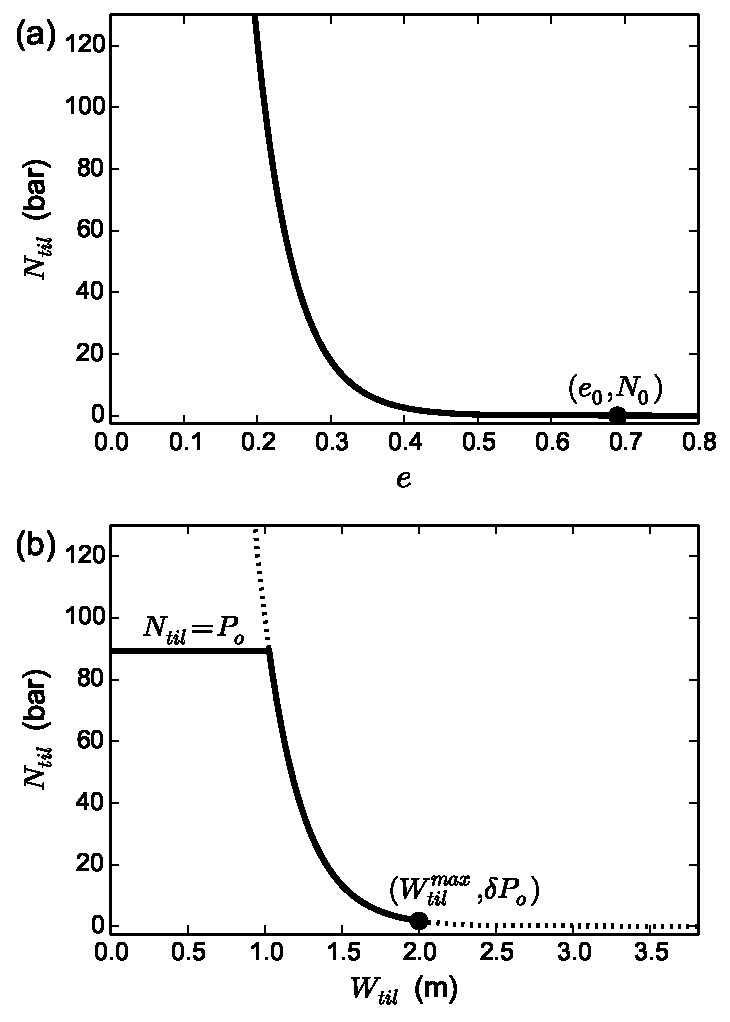
\includegraphics[width=3.0in,keepaspectratio=true]{Ntilfunctions}
\caption{\textbf{(a)} Equation \eqref{eq:voidpressureexponential} determines the effective pressure $\Ntil$ as a function of the void ratio $e$.  Reference values $e_0=0.69$, $N_0=10^3$ Pa used by \cite{Tulaczyketal2000} are indicated.  \textbf{(b)}  In this paper we parameterize the amount of till-stored water by a thickness $\Wtil$ instead of $e$, so $\Ntil$ is a function of $\Wtil$ (dotted).  Furthermore the effective pressure $\Ntil$ is bounded above by overburden pressure $P_o$ and below by a fixed fraction $\delta$ of $P_o$, as shown here in the case of 1000 meters ice thickness, $\delta = 0.02$, and $\Wtilmax=2.0$ meters; see text.  At the lower bound, excess water is ``dumped'' into the transport system.}
\label{fig:Ntilfunctions}
\end{figure}

\subsection{Effective pressure on the till}  There is extensive evidence that deformation of saturated till is well-modeled by a plastic (Coulomb friction) or nearly-plastic rheology \citep{Hookeetal1997,TrufferHarrisonEchelmeyer2000,Tulaczyketal2000,SchoofTill}.  The yield stress $\tau_c$ of the saturated till satisfies the Mohr-Coulomb relation
\begin{equation}
\tau_c = c_0 + (\tan \varphi) \Ntil  \label{eq:mohrcoulomb}
\end{equation}
where $c_0$ is the till cohesion, $\varphi$ is the till friction angle, and $\Ntil$ is the effective pressure of the overlying ice on the saturated till \citep{CuffeyPaterson}.\footnote{The effective pressure $N=P_o-P$ used in the next section for modeling cavity closure is distinct from $\Ntil$.  This distinction is justified by the very low hydraulic conductivity of till.  Also, the till effective pressure $\Ntil$ does not affect the model for the horizontal transport of water.}

Let $e = V_w / V_s$ be the till void ratio, where $V_w$ is the volume of water in the pore spaces and $V_s$ is the volume of mineral solids \citep{Tulaczyketal2000}.  From the standard theory of soil mechanics and laboratory experiments on till \citep{Hookeetal1997,Tulaczyketal2000}, a linear relation exists between the logarithm of $\Ntil$ and $e$,
\begin{equation}
e = e_0 - C_c \log_{10}\left(\Ntil / N_0\right).  \label{eq:voidpressure}
\end{equation}
Here $e_0$ is the void ratio at a reference effective pressure $N_0$ and $C_c$ is the coefficient of compressibility of the till.  Equivalently, \eqref{eq:voidpressure} is an exponential function determining $\Ntil$ from $e$ \citep[equation (15)]{vanderWeletal2013}:
\begin{equation}
\Ntil = N_0 10^{(e_0 - e)/C_c}.  \label{eq:voidpressureexponential}
\end{equation}
Figure \ref{fig:Ntilfunctions}(a) shows a graph of \eqref{eq:voidpressureexponential}.  Note that in \eqref{eq:voidpressure} and \eqref{eq:voidpressureexponential}, $\Ntil=0$ is not achieved for finite values of the void ratio $e$.

While equations \eqref{eq:voidpressure} or \eqref{eq:voidpressureexponential} suggest that the effective pressure could be any positive number, in fact the area-averaged value of $\Ntil$ under ice sheets and glaciers has limits.  It cannot exceed the overburden pressure for any sustained period.  Furthermore our model of subglacial water movement is that once the till is close to its maximum capacity then the excess water will be ``dumped'' into a transport system.  We suppose this occurs at a small, fixed fraction of the overburden pressure.  Thus we assume bounds
\begin{equation}
\delta P_o \le \Ntil \le P_o  \label{eq:Ntilbounds}
\end{equation}
where $\delta = 0.02$ in the experiments in this paper.

The void ratio $e$ and the effective water layer thickness $\Wtil$ are describing the same thing.  In fact, if $\Delta x$, $\Delta y$ are the horizontal dimensions of a rectangular patch of till then $V_w = \Wtil \,\Delta x \,\Delta y$ and $V_s = \eta \,\Delta x \,\Delta y$ where $\eta$ is the thickness of the mineral portion of the till.\footnote{In equation \eqref{eq:voidpressureexponential} the value $e=0$ would give $\Ntil=N_0 10^{e_0/C_c} \approx 6000\, \text{bar}$.  Thus we could say that $\eta$ is the till thickness if compressed to zero void ratio, but the needed pressure is much larger than attained under an ice sheet.}  Because $e=V_w/V_s$,
\begin{equation}
e = \frac{\Wtil}{\eta}.  \label{eq:voidequivalent}
\end{equation}
On the other hand we will describe the maximum capacity of the till by specifying a maximum on the water layer thickness \citep{BBssasliding}, that is,
\begin{equation}
0 \le \Wtil \le \Wtilmax.  \label{eq:Wtilbounds}
\end{equation}
Because the minimum of the effective pressure $\Ntil$ occurs at the maximum void ratio $e$, and by \eqref{eq:voidequivalent} this maximum occurs when $\Wtil$ is maximum, equations \eqref{eq:voidpressure}, \eqref{eq:Ntilbounds}, and \eqref{eq:voidequivalent} combine to express the solid-till thickness $\eta$ in terms of our preferred parameters and the overburden pressure,
\begin{equation}
\eta = \frac{\Wtilmax}{e_0 - C_c \log_{10}\left(\delta P_o / N_0\right)}.  \label{eq:etaexpression}
\end{equation}
FIXME:  write $\Ntil(\Wtil)$ as consequence, and refer to Figure 1(b)
\begin{equation}
FIXME \Ntil = \min\left\{P_o,\, \delta P_o \, 10^{(e_0/C_c) \left(1 - (\Wtil/\Wtilmax)\right)}\right\}. \label{eq:Wtilpressure}
\end{equation}
Compare equation (15) in \cite{vanderWeletal2013}.

It follows from equations \eqref{eq:mohrcoulomb} and \eqref{eq:Wtilpressure} that the till yield stress $\tau_c$ can be determined from the water amount $\Wtil$.  The Mohr-Coulomb relation \eqref{eq:mohrcoulomb} is, therefore, a function $\tau_c(\Wtil)$.  Regarding the parameters in this relation, we note:
\renewcommand{\labelenumi}{(\emph{\roman{enumi}})}
\begin{enumerate}
\item Experiments on till suggest small values for cohesion, $0 \le c_0 \lesssim 1$ kPa \citep{Tulaczyketal2000}, and we choose $c_0=0$ for concreteness.
\item Observed till friction angles $\varphi$ are in a $18^\circ$--\,$40^\circ$ range \citep{CuffeyPaterson}.  The spatial variability of this parameter can be assumed to be large and unknown.  Simulations of the whole Antarctic \citep{Martinetal2011} and Greenlandic \citep{AschwandenAdalgeirsdottirKhroulev} ice sheets have been based on a hypothesis that the till friction angle $\varphi$ can depend on bed elevation, so as to accommodate the submarine history of some sediments.
\item The ratio $e_0/C_c$ can be determined by laboratory experiments on till samples \citep[e.g.][]{Hookeetal1997,Tulaczyketal2000}.  Values for the dimensionless constants $e_0$ and $C_c$ used in this paper are from till samples from ice stream B in Antarctica, namely $e_0=0.69$ and $C_c=0.12$ in Figure 6 of \cite{Tulaczyketal2000}, thus $e_0/C_c=5.75$.
\item The maximum capacity parameter $\Wtilmax$ could be set in a location-dependent manner from in situ \citep{Tulaczyketal2000} or seismic reflection \citep{Rooneyetal1987} evidence, but for simplicity we set it to a constant value of $2$ meters.
\end{enumerate}

\subsection{Sliding law}  Ice sliding velocity is determined by solving a stress balance in which the vector basal shear stress $\boldsymbol\tau_b$ appears as a boundary condition or term in the balance \citep{SchoofStream,SchoofCoulombBlatter,BBssasliding}.  In PISM the scalar yield stress $\tau_c$ determines the basal shear stress through a sliding law
\begin{equation}
\boldsymbol\tau_b = - \tau_c \frac{\mathbf{u}}{|\mathbf{u}|^{1-q} u_0^q} \label{eq:pseudobasalstress}
\end{equation}
where $\mathbf{u}$ is the sliding velocity of the base of the ice, $0\le q \le 1$ , and $u_0$ is a threshold sliding velocity \citep{AschwandenAdalgeirsdottirKhroulev}.  Power law \eqref{eq:pseudobasalstress} generalizes, and includes as the case $q=0$, the purely-plastic (Coulomb) relation $\boldsymbol\tau_b = - \tau_c \mathbf{u}/|\mathbf{u}|$.  At least in the $q\ll 1$ cases, under \eqref{eq:pseudobasalstress} the till ``yields'' and the magnitude of the basal shear stress becomes nearly independent of the sliding speed $|\mathbf{u}|$ as it becomes larger than the threshold $u_0$.  Equation \eqref{eq:pseudobasalstress} could also be written in generic power-law form $\boldsymbol\tau_b = - \beta |\mathbf{u}|^{q-1} \mathbf{u}$ with coefficient $\beta = \tau_c / u_0^q$; this includes the linear case $q=1$ in which we have $\beta = \tau_c/u_0$.


\section{Capacity of a linked-cavity distributed system} \label{sec:capacity}

The evolution of the area-averaged thickness of the cavities in a distributed linked-cavity system can be described as the difference of opening and closing rates \citep{Hewitt2011}.  This thickness $Y$, also called the bed separation \citep{Bartholomausetal2011}, has evolution equation
\begin{equation}
\frac{\partial Y}{\partial t} = \mathcal{O}(|\bv_b|,Y) - \mathcal{C}(N,Y) \label{eq:hewittcapacity}
\end{equation}
where $\bv_b$ is the ice base (sliding) velocity and $N=P_o-P$ is the effective pressure on the cavity system.  Denoting $X_+= \max\{0,X\}$, as in \cite{Schoofetal2012} we choose an opening term based on cavitation only:
\begin{equation}
\mathcal{O}(|\bv_b|,Y) = c_1 |\bv_b| (W_r - Y)_+. \label{eq:openingform}
\end{equation}
Here $W_r$ is a maximum roughness scale of the basal topography and $c_1$ is a constant.  The closing term models ice creep only \citep{Hewitt2011,Schoofetal2012}:
\begin{equation}
\mathcal{C}(N,Y) = c_2 A N^3 Y. \label{eq:closingform}
\end{equation}
Here $A$ is the ice softness and $c_2$ is a constant which must be constrained by observations.  We have used Glen exponent $n=3$ for concreteness and simplicity.

Equation \eqref{eq:hewittcapacity} describes the evolution of the upper surface of the subglacial cavities.  By \eqref{eq:openingform} the opening term $\mathcal{O}$ is nonnegative.  The closing term $\mathcal{C}$ in \eqref{eq:closingform} is also nonnegative because our modeled pressure $P$ satisfies bounds $0\le P \le P_o$.  The opening and closing terms \eqref{eq:openingform} and \eqref{eq:closingform} satisfy the inequalities (2.5)--(2.7) in \cite{Schoofetal2012}.

The physical intuition behind a pressure model which combines \eqref{eq:hewittcapacity} with mass conservation \eqref{eq:conserve} and a Darcy flux relation like \eqref{eq:flux} is as follows.  If the cavity is larger than local water sources can immediately fill then the pressure should drop.  Lower pressure encourages water inflow and, by \eqref{eq:closingform}, it speeds cavity closure, bringing the pressure back up.  Conversely, if local water sources exceed capacity then increased pressure should push water out of the area, and also creep closure slows.  This ``intuition'' requires a pressure closure, however, which is addressed in the next section.


\section{Closures to determine pressure} \label{sec:closures}

At this point we do not know how to compute the water pressure $P$ given the other variables and data of the problem, namely $b$, $H$, $m$, $|\bv_b|$, $W$, $\Wtil$, and $Y$.  The evolution equations listed so far, namely \eqref{eq:adeqn}, \eqref{eq:tilldynamics}, and \eqref{eq:hewittcapacity}, can be simplified to three equations in the four unknown state variables $W$, $\Wtil$, $Y$, and $P$.   A closure is needed.

\subsection{Simplified closures without cavity evolution}  We first consider two simple closures which appear in the literature but which do not use cavity evolution equation \eqref{eq:hewittcapacity} or similar physics.  These simplified closures differ in their physical motivation and the form of their mass conservation equations.  We list them because the resulting simplified conservation equations emerge as steady-state reductions of our more complete theory.  For simplicity we present them without till storage, that is, with $\Wtilmax=0$ in previous equations.  We state only the constant conductivity case ($\alpha=1$ and $\beta=2$ in equation \eqref{eq:flux}).

Setting the pressure equal to the overburden pressure is the simplest closure \citep{LeBrocqetal2009,Shreve1972}:
\begin{equation}
P = P_o.\label{eq:Pisoverburden}
\end{equation}
This model is sometimes used for ``routing'' subglacial water under ice sheets so as to identify subglacial lake locations \citep{Livingstoneetal2013,Siegertetal2009}.  Straightforward calculations using equations \eqref{eq:conserve}, \eqref{eq:flux}, and \eqref{eq:Pisoverburden} show that the advection-diffusion form \eqref{eq:adeqn} has an ice-geometry-determined velocity,
\begin{equation}
  \frac{\partial W}{\partial t} = - \Div\left(\tilde\bV\, W\right) + \Div\left(\rho_w g k \,W\, \grad W\right) + \frac{m}{\rho_w}   \label{eq:PisoverConservation}
\end{equation}
where
\begin{equation}
\tilde\bV = - \rho_w g k \left[\frac{\rho_i}{\rho_w} \grad h + \left(1-\frac{\rho_i}{\rho_w}\right) \grad b\right].
\end{equation}

Because the approximation $W\ll H$ is usually accepted, so that the hydraulic potential is insensitive to the water layer thickness, i.e.~$\psi = P_o + \rho_w g b$ \citep{LeBrocqetal2009}, the diffusion term $\Div\left(\rho_w g k \,W\, \grad W\right)$ on the right of \eqref{eq:PisoverConservation} is usually not included.  With this common simplification, equation \eqref{eq:PisoverConservation} becomes a pure advection with a velocity $\tilde\bV$ which is independent of $W$.  It therefore possesses characteristic curves \citep{Evans} which are the \emph{a priori} known trajectories of the water flow.  These trajectories are determined by ice sheet geometry.

However, without a diffusion term equation \eqref{eq:PisoverConservation} exhibits continuum solutions with infinite water concentration at every location where the simplified potential $\psi = P_o + \rho_w g b$ has a minimum.  In fact, applications using the simplified potential tend to only compute the characteristic curves \citep[i.e.~``pathways'',][]{Livingstoneetal2013} and not the evolving field $W$.  We therefore prefer equation \eqref{eq:PisoverConservation} as stated, \emph{with} the diffusion term, because it is well-posed for positive initial and boundary values on $W$ \citep[compare][]{Hewittetal2012}.  Continuum solutions have finite water layer thickness at all times and solutions will converge under sufficient grid refinement.

At an almost opposite extreme in terms of the mathematical form, the second simplified closure we consider assumes that the water pressure is locally determined by the amount of water.  Specifically, \cite{FlowersClarke2002_theory} propose
\begin{equation}
P_{FC}(W) = P_o \left(\frac{W}{W_{\text{crit}}}\right)^{7/2}. \label{eq:PofWFC}
\end{equation}
For Trapridge glacier \cite{FlowersClarke2002_trapridge} use $W_{\text{crit}}=0.1$ m.  Because of the local relation between water amount and pressure, implementation of a coupled ice flow and subglacial hydrology model is simplified because no pressure evolution equation needs to be solved \citep{PimentelFlowersSchoof2010,PimentelFlowers2011}.  One obvious concern with form \eqref{eq:PofWFC} is that $P_{FC}(W)$ can be arbitrarily larger than overburden pressure for large amounts of water \citep{Schoofetal2012}.

In the flat bedrock case $\grad b = 0$, we can derive an equation from \eqref{eq:conserve}, \eqref{eq:flux}, and \eqref{eq:PofWFC}, namely
\begin{equation}
\frac{\partial W}{\partial t} =  \Div \left(k\,W \grad P_{FC}(W)\right) + \frac{m}{\rho_w}. \label{eq:PofWFCConservation}
\end{equation}
Equation \eqref{eq:PofWFCConservation} is a nonlinear diffusion which generalizes the porous-medium equation $\partial W/\partial t = \grad^2 (W^\gamma)$ \citep{Schoofetal2012,VazquezPME}.  The main idea in such a nonlinear diffusion is that the direction of the flux is $-\grad W$.  Physically, however, it would seem that $\bq \sim -\grad \psi$ would give flux directions different from $-\grad W$ in many cases, especially in rapidly-evolving hydrologic systems.

\subsection{Full-cavity closure}  Requiring the subglacial layer to be full of water is a closure for the subglacial pressure $P$.  We adopt it in our model:
\begin{equation}
W = Y.\label{eq:strongclosure}
\end{equation}
The consequences of this closure are explored at some length by \cite{Schoofetal2012}, \cite{Hewittetal2012}, and \cite{Werderetal2013}.  They describe the case where cavities are full as the ``normal pressure'' condition (e.g.~equation (4.13) in \cite{Schoofetal2012}).

Equation \eqref{eq:strongclosure} obviously allows us to eliminate either $W$ or $Y$ as a state variable.  We choose to eliminate $Y$ because $W$ is part of the conserved mass $W + \Wtil$.  Using equations \eqref{eq:conserve}, \eqref{eq:hewittcapacity}, and \eqref{eq:strongclosure} we can derive
\begin{equation}
\mathcal{O}(|\bv_b|,W) - \mathcal{C}(N,W) + \ddt{\Wtil} + \Div\bq = \frac{m}{\rho_w}. \label{eq:elliptic}
\end{equation}
In the zero till storage case (set $\Wtilmax=0$ so $\Wtil=0$), equation \eqref{eq:elliptic} is exactly the elliptic pressure equation (2.12) of \cite{Schoofetal2012}.  Given values for the water amount $W$, they solve \eqref{eq:elliptic} with pressure boundary conditions at the lateral edges of the subglacial hydrologic system to determine the pressure $P$.

\cite{Schoofetal2012} argue that a model based on \eqref{eq:elliptic} should accommodate the possibility of partially-empty cavities with $W<Y$ and at zero pressure $P=0$.  As evidence for vapor/air-filled cavities does not exist underneath tidewater glaciers or ice sheets, though of course subglacial hydrology is poorly-observed generally, we accept a potential loss of model completeness by using a full-cavity model.  An overpressure condition $P>P_o$ has been observed in ice sheets \citep[for example]{Dasetal08}, but only for short durations.  Unlike \cite{Werderetal2013}, our modelled pressure satisfies $P\le P_o$, as would the computationally-expensive elliptic variational inequality model of \cite{Schoofetal2012}. 

\subsection{Notional englacial porosity as a regularization}  Englacial systems of cracks, crevasses, and moulins have been observed in glaciers \citep[for example]{Fountainetal2005,Bartholomausetal2008,Harperetal2010}, and these have been included in combined englacial/subglacial hydrology models \citep{FlowersClarke2002_theory,Bartholomausetal2011,Hewitt2013,Werderetal2013}.  The englacial system is generally parameterized as having macroporosity $0\le \phi < 1$.  If the englacial system is efficiently-connected to the subglacial water then the amount of englacial water is equivalent to the subglacial pressure.  Thus, in such an englacial hydrologic system, higher or lower subglacial pressure is reflected by higher or lower ``water table.''

\cite{Bueler2014correspondence} shows that an extension of the lumped englacial/subglacial model in \cite{Bartholomausetal2011} to the distributed case gives an equation similar to \eqref{eq:elliptic}, but with the crucial difference that the equation is parabolic for the pressure and not elliptic (compare \cite{Hewittetal2012}).  The time-derivative term is proportional to the englacial porosity $\phi$.  Based on this re-analysis of \cite{Bartholomausetal2011}, we use this parabolic equation in our model with constant notional englacial porosity $\phi=\phi_0$:
\begin{align}
\frac{\phi_0}{\rho_w g} \ddt{P} &= - \Div \bq + \frac{m}{\rho_w} + \mathcal{C}(N,W)  \label{eq:regpressureequation} \\
  &\qquad\qquad - \mathcal{O}(|\bv_b|,W) - \ddt{\Wtil}. \notag
\end{align}
Compare equations (7) in \cite{Hewitt2013} and (24) in \cite{Werderetal2013}.

Addition of englacial porosity to the model allows a user-adjustable trade-off between temporal detail in the pressure evolution versus computational effort \citep{vanPeltthesis}.  If the englacial porosity $\phi_0$ is small, so that there is a nearly impermeable ``cap'' on the subglacial system, as would occur under a thick ice sheet, then equation \eqref{eq:regpressureequation} is \emph{stiff} and indeed similar, in terms of numerical solution, to an elliptic equation.  However, if $\phi_0$ is relatively large then equation \eqref{eq:regpressureequation} causes local changes in subglacial pressure $P$ to be damped in the speed and range of their influence on other parts of the connected subglacial hydrologic system.

In fact, equation \eqref{eq:regpressureequation} is stiff to a degree inversely-proportional to $\phi_0$, in the sense that the diffusive range of pressure evolution is proportional to $\phi_0$.  The \cite{Schoofetal2012} theory is the infinitely-stiff $\phi_0=0$ case.  In general, stiffer equations are harder to solve numerically, and differential-algebraic equations like the system of the mass conservation equation and the elliptic equation \eqref{eq:elliptic} are the hardest \citep{AscherPetzold}.

\cite{Schoofetal2012} show that the time-independent mathematical problem encompassing \eqref{eq:elliptic} (in the $\Wtilmax=0$ case), constraints \eqref{eq:bounds}, and appropriate pressure boundary conditions can be written as an elliptic variational inequality \citep{KinderlehrerStampacchia}.  This variational inequality problem is asserted to be ``numerically prohibitive'' by \cite{Werderetal2013} when solved in two dimensions at each step of a time-stepping model.  Instead, in our model we have an explicit time-stepping scheme---see section \ref{sec:num}---with adaptive time-stepping to satisfy stability conditions.

Stiffness of pressure equation \eqref{eq:regpressureequation} follows from the incompressibility of water and the relative non-distensibility (i.e.~hardness) of the ice and bedrock.  \cite{Clarke2003} addresses stiffness in a physically-different but related way by including in his subglacial water equation a relaxation (damping) parameter  ``$\beta$'' which is based on the small compressibility of water, but which is more than two orders of magnitude larger than the physical value.  Clarke's parameter $\beta$ appears in his equation exactly as the englacial porosity $\phi_0$ appears in equation \eqref{eq:regpressureequation}, multiplying the pressure time derivative.

Equation \eqref{eq:regpressureequation} for $P$ is coupled to the advection-diffusion equation \eqref{eq:adeqn} for $W$.  Section \ref{sec:num} gives a quantitative analysis of the time-scales related to solving \eqref{eq:adeqn} and \eqref{eq:regpressureequation} together.


\section{A new subglacial hydrology model in PISM} \label{sec:newmodel}

\subsection{Summary of equations and symbols}  The major, coupled equations for the model are \eqref{eq:adeqn}, \eqref{eq:mohrcoulomb}, \eqref{eq:tilldynamics}, and \eqref{eq:regpressureequation}.  Collected here for clarity they are:
\begin{align}
&\ddt{W} + \ddt{\Wtil} = - \Div\left(\bV\, W\right) + \Div \left(D \grad W\right) + \frac{m}{\rho_w}, \label{eq:bluebox} \\
&\tau_c = c_0 + (\tan \varphi)\, \Ntil, \notag \\
&FIXME \Ntil = \min\left\{P_o,\, \delta P_o \, 10^{(e_0/C_c) \left(1 - (\Wtil/\Wtilmax)\right)}\right\}, \notag \\
&\frac{\partial \Wtil}{\partial t} = \frac{m}{\rho_w} - C_d, \notag \\
&\frac{\phi_0}{\rho_w g} \ddt{P} + \ddt{\Wtil} = - \Div\left(\bV\, W\right) + \Div \left(D \grad W\right) + \frac{m}{\rho_w} \notag \\
& \qquad \qquad \qquad + c_2 A (P_o - P)^3 W - c_1 |\bv_b| (W_r - W)_+. \notag
\end{align}
The model also includes bounds on the state variables, namely $0\le W$, $0\le \Wtil \le \Wtilmax$, and $0 \le P \le P_o$.  We also require these associated functions, recollected here:
\begin{align*}
K    &= k W^{\alpha-1} \left|\grad(P+\rho_w g b)\right|^{\beta-2} && \text{effective conductivity} \\
\bV  &= - K \grad\left(P + \rho_w g b\right) && \text{velocity of $W$} \\
D    &= \rho_w g K W && \text{diffusivity of $W$} \\
P_o  &= \rho_i g H && \text{overburden pressure}.
\end{align*}

\begin{table*}[ht]
\caption{Time- and space-dependent functions in subglacial hydrology model \eqref{eq:bluebox}, including symbol, units, and meaning.}
\begin{tabular}{l|l}
\hline
\emph{state functions} & \begin{tabular}{lll}
        $W$ & m \phantom{llllllllllll\,} & effective thickness of transportable water \\
        $\Wtil$ & m & effective thickness of water stored in till \\
        $P$ & Pa & pressure of transportable water \\
        \end{tabular} \\ \hline
\emph{data functions} &  \begin{tabular}{lll}
        $b$ & m & bedrock elevation \\
        $\varphi$ &  & till friction angle \\
        $H$ & m & ice thickness \\
        $m$ & $\text{kg}\,\text{m}^{-2}\,\text{s}^{-1}$ & total melt water input into subglacier \\
        $|\bv_b|$ & $\text{m}\,\text{s}^{-1}$ & ice sliding speed \\
        \end{tabular} \\ \hline
\emph{output} &  \begin{tabular}{lll}
        $\Ntil$ & Pa & effective pressure on the till \\
        $\tau_c$ \phantom{l\;} & Pa \phantom{llllllllllll} & till yield stress \\
        \end{tabular} \\ \hline
\end{tabular}
\label{tab:symbols}
\end{table*}

\begin{table*}[ht]
  \centering
  \caption{Physical constants and model parameters.  Default values are overridden in some experiments.}
  \begin{tabular}{lllp{3.0in}} 
    \textbf{Name} & \textbf{Default Value} & \textbf{Units} & \textbf{Description}\\
\hline
    $A$ & $3.1689\times 10^{-24}$ & $\text{Pa}^{-3}\,\text{s}^{-1}$ & ice softness \citep{EISMINT96} \phantom{$\Big|$} \\
    $\alpha$ & $5/4$ & & power in flux formula  \citep{Schoofetal2012} \\
    $\beta$ & $3/2$ & & power in flux formula  \citep{Schoofetal2012} \\
    $c_0$ & 0 & Pa & till cohesion \citep{Tulaczyketal2000} \\
    $c_1$ & $0.5$ & $\text{m}^{-1}$ & cavitation coefficient \citep{Schoofetal2012} \\
    $c_2$ & $0.04$ & & creep closure coefficient \\
    $C_c$ & 0.12 &  & till compressibility \citep{Tulaczyketal2000} \\
    $C_d$ & $0.001$ &  $\text{m}\,\text{a}^{-1}$ & background till drainage rate \\
    $\delta$ & 0.02 &  & fraction of overburden pressure \\
    $e_0$ & 0.69 &  & reference void ratio at $N_0$ \citep{Tulaczyketal2000} \\
    $\phi_0$ & $0.01$ & & notional (regularizing) englacial porosity \\
    $g$ & $9.81$ & m $\text{s}^{-2}$ & acceleration of gravity \\
    $k$ & $0.001$ & $\text{m}^{2\beta-\alpha} \text{s}^{2\beta-3} \text{kg}^{1-\beta}$ & conductivity coefficient \citep{Schoofetal2012} \\
    $N_0$ & $10^3$ & Pa & reference effective pressure \citep{Tulaczyketal2000} \\
    $\rho_i$ & $910$ & $\text{kg}\,\text{m}^{-3}$ & ice density \citep{GreveBlatter2009} \\
    $\rho_w$ & $1000$ & $\text{kg}\,\text{m}^{-3}$ & fresh water density \citep{GreveBlatter2009} \\
    $W_r$ & $0.1$ & $\text{m}$ & roughness scale \citep{Hewittetal2012} \\
    $\Wtilmax$ & $2\phantom{\Big|}$ & $\text{m}$ & maximum water in till \citep{BBssasliding} \\
    \hline
  \end{tabular}
 \label{tab:constants}
\end{table*}

Model equations \eqref{eq:bluebox} relate the state functions, data functions, and output function listed in Table \ref{tab:symbols} to the physical constants and model parameters in Table \ref{tab:constants}.  Only the state functions must be provided with initial values, and only they must be saved when stopping and restarting a time-stepping numerical model.  The ``data'' functions are either supplied by observations or by other components an ice sheet model (e.g.~the stress balance in an ice dynamics model will provide $|\bv_b|$).

The yield stress function $\tau_c$ is the most important output of the model.  It determines the basal shear stress used in the stress balance equations of an ice dynamics model.  Full two-way coupling would include the ice dynamics model passing fields $b$, $H$, $m$, and $|\bv_b|$ to the subglacial hydrology model, and $\tau_c$ passed in the other direction.

The model parameters in Table \ref{tab:constants} are all constant (i.e.~time- and space-independent) in the current paper but they could be allowed to vary spatially if desired.  Exploration of the parameter space represented by Table \ref{tab:constants} is important, but essentially it is beyond the scope of this model-description paper.

\subsection{Reduction to existing models}  Four reductions (limiting cases) of model \eqref{eq:bluebox} can now be stated precisely:

\renewcommand{\labelenumi}{\textbf{(\roman{enumi})}}
\begin{enumerate}
\item The zero till storage ($\Wtilmax=0$) and zero englacial porosity ($\phi_0=0$) case of \eqref{eq:bluebox} is the model described by \cite{Schoofetal2012}, recalling that $\bq = - K W \grad \psi$,
\begin{align}
&\frac{\partial W}{\partial t} = - \Div\left( K W \grad \psi \right) + \frac{m}{\rho_w}, \label{eq:schoofsmodel} \\
&0 = \Div \left( K W \grad \psi \right) + \frac{m}{\rho_w} \notag \\
&\qquad \qquad + c_2 A (P_o - P)^3 W - c_1 |\bv_b| (W_r - W)_+.  \notag
\end{align}
The bounds $W \ge 0$ and $0 \le P \le P_o$ are unchanged.  Model \eqref{eq:bluebox} is a parabolic regularization of \eqref{eq:schoofsmodel} based on a notional connection to porous englacial storage, with a small porosity parameter $\phi_0$, and with coupling to additional till storage; see section \ref{sec:closures}.

\item The $P=P_o$ limit of \eqref{eq:bluebox}, in which physical processes for the evolution of pressure are ignored, is the standard model for ``routing'' water to subglacial lakes under cold ice sheets \citep{Siegertetal2009,Livingstoneetal2013}.  Assuming again that till storage is removed ($\Wtilmax=0$) then the model has only $W$ as a state variable.

The single evolution equation of this reduced model is
\begin{equation}
\frac{\partial W}{\partial t} = - \Div\left(\bV\, W\right) + \Div \left(D \grad W\right) + \frac{m}{\rho_w}. \label{eq:lakesmodel}
\end{equation}
along with the bound $W \ge 0$ and definitions $K = k W^{\alpha-1} \left|\grad (P_o + \rho_w g b)\right|^{\beta-2}$ and $\bV = - K \grad \left(P_o + \rho_w g b\right)$.  As noted in section \ref{sec:closures}, the $\alpha=1$ case of this model routes water with a velocity which is determined entirely by ice and bedrock geometry.  Thus this reduced model is essentially an advection, but, because of \eqref{eq:potential} for the hydraulic potential, giving some diffusion, model \eqref{eq:lakesmodel} is well-posed and has continuous solutions.  Equation \eqref{eq:lakesmodel} therefore represents a modest improvement to the ``routing'' models \citep{Siegertetal2009,Livingstoneetal2013}.

\item The non-distributed ``lumped'' form of \eqref{eq:bluebox}, in which, in particular, $\Div \bq = (q_{out} - q_{in})/L$ where $L$ is the length of the glacier and $q_{out},q_{in}$ are given by observations, is the porous glacier model of \cite{Bartholomausetal2011}.  The correspondence is further explained in \cite{Bueler2014correspondence}, with an emphasis on the pressure equation which applies in that lumped model.

\item The undrained plastic bed (UPB) model of \cite{Tulaczyketal2000b} arises as the $W=0,\bq=0,\phi_0=0$ reduction of \eqref{eq:bluebox}:
\begin{align}
&\ddt{\Wtil} = \frac{m}{\rho_w}, \label{eq:upbbox} \\
&\tau_c = c_0 + (\tan \varphi)\, \Ntil, \notag \\
&FIXME \Ntil = N_0 \, 10^{(e_0/C_c) \left(1 - (\Wtil/\Wtilmax)\right)}, \notag
\end{align}

The UPB model depends on friction-heating feedback to keep $\Wtil$ bounded, which does not work in a membrane-stress-inclusive theory, in which local friction heating is a non-local function of changes in till strength.  \cite{BBssasliding} therefore enforce $\Wtil \le \Wtilmax$ by non-conservatively removing water that would raise $\Wtil$ above the bound, which is a minimal ``drained'' version of the UPB model.
\end{enumerate}

The above list does not imply that all possible subglacial hydrology models are subsumed in ours.  For example, the subglacial hydrology model of \cite{JohnsonFastook} could be considered as a variation on idea \textbf{(ii)} above but it cannot be considered a reduction of our model.  The \cite{FlowersClarke2002_theory} model is also not a reduction, although a significant connection is explained in the next section on steady states.

Most significantly, models which include conduits \citep[among others]{Schoofmeltsupply,PimentelFlowers2011,Hewittetal2012} are not reductions of our model.  Conduit evolution is numerically-straightforward to implement in one-dimensional hydrology models \citep{PimentelFlowers2011,Hewittetal2012,vanderWeletal2013} but when extended to two-horizontal dimensions all existing models \citep{Schoofmeltsupply,Hewitt2013,Werderetal2013} become ``lattice'' models without a known continuum limit.


\section{Analysis of steady states}  \label{sec:steady}

\subsection{Equations of steady state}  The steady states of equations \eqref{eq:bluebox} are of physical modelling importance because the subglacial system can be close to steady state much of the time.  In steady state several physical processes become decoupled.  In fact we can make four specific observations which are special to steady state, and which we find are useful in understanding the time-dependent model:
\renewcommand{\labelenumi}{(\emph{\roman{enumi}})}
\begin{enumerate}
\item there is a functional relationship $P=P(W)$ which determines the pressure given the water amount,
\item the apparently advective flux ``$\bV W$'' actually acts diffusively if sliding is occurring and the water amount is either small or is comparable to the roughness scale,
\item the water amount generally scales inversely with the conductivity ($W \sim 1/k$), and
\item exact solutions can be constructed.
\end{enumerate}
In this section we address (\emph{i}), (\emph{ii}), and (\emph{iii}), while (\emph{iv}) is addressed in section \ref{sec:exactsolution}.

We simplify the model slightly before addressing steady states: fix $\alpha=1$ and $\beta=2$, and remove till storage by setting $\Wtilmax=0$.  The general observations above will apply without these simplifications, but the formulas here are more manageable because of them.

The steady form of model \eqref{eq:bluebox}, with these simplifications, can be written as follows in terms of $\bV,\bq,W,P$:
\begin{align}
\bV &= - k \grad \left(P + \rho_w g b\right), \label{eq:Vsteady} \\
\bq &= \bV W - \rho_w g k W \grad W, \label{eq:qsteady} \\
0 &= - \Div \bq + \frac{m}{\rho_w}, \label{eq:masscontsteady} \\
0 &= c_2 A (P_o - P)^3 W - c_1 |\bv_b| (W_r - W)_+. \label{eq:openclosesteady}
\end{align}
Note that we also have bounds $W\ge 0$ and $0 \le P \le P_o$.

Steady state equations \eqref{eq:Vsteady}--\eqref{eq:openclosesteady} are stated in the one-dimensional case by \cite{Schoofetal2012} model, where the decoupling is also noted; see equations (5.8) and (5.10) in \citep{Schoofetal2012}.

\subsection{Pressure as a function of $W$ in steady state}  Relative to the time-dependent form \eqref{eq:bluebox}, we see there are separate balances between the divergence of the flux and the water input on the one hand (equation \eqref{eq:masscontsteady}), and the opening and closing processes on the other hand (equation \eqref{eq:openclosesteady}).  The latter balance allows us to write the pressure $P=P(W)$ in steady state as a continuous function of the water amount $W$.

Steady state is only possible if a condition holds:
\begin{equation}
c_1 |\bv_b| (W_r - W)_+ \le c_2 A P_o^3 W. \label{eq:steadyboundfirst}
\end{equation}
The reason for this constraint combines the cavity evolution equation \eqref{eq:hewittcapacity}, in the steady state case, and the full-cavity closure \eqref{eq:strongclosure}, giving \eqref{eq:openclosesteady}.  But \eqref{eq:openclosesteady} is only possible if the maximum closing rate $\mathcal{C}(N,W)$, which depends on pressure $P$, can match the opening rate $\mathcal{O}(|\bv_b|,W)$, which is pressure-independent.  The maximum closure rate occurs at zero water pressure, thus \eqref{eq:steadyboundfirst}.

We define the following scaled basal sliding speed which has units of pressure:
\begin{equation}
s_b =  \left(\frac{c_1 |\bv_b|}{c_2 A}\right)^{1/3}.  \label{eq:definesb}
\end{equation}
One regard $s_b$ as a scale for the pressure drop from cavitation.  Then \eqref{eq:steadyboundfirst} is equivalent to
\begin{equation}
W \ge W_c := \frac{s_b^3}{s_b^3 + P_o^3} W_r. \label{eq:steadyboundsecond}
\end{equation}
If \eqref{eq:steadyboundfirst} or \eqref{eq:steadyboundsecond} holds then
\begin{equation}
P(W) = P_o - s_b \left(\frac{(W_r - W)_+}{W}\right)^{1/3}.  \label{eq:PofWsteady}
\end{equation}
Note that in \eqref{eq:PofWsteady} we have $P(W_c)=0$.  Underpressure ($P=0$) with subcritical water amount ($W<W_c$) does not occur in steady state though it can occur in nonsteady conditions.  Formula \eqref{eq:PofWsteady} may apply even if $W\ge W_r$, in which case the water pressure takes the overburden value $P = P_o$.

\newcommand{\upto}{ \!\!\nearrow\! }
\newcommand{\downto}{ \!\searrow\! }
Figure \ref{fig:psteady-vb} shows the function $P(W)$ from \eqref{eq:PofWsteady} for different values of sliding speed $|\bv_b|$, and Figure \ref{fig:psteady-Po} for values of overburden pressure $P_o$.  We see that as the water amount reaches the roughness scale ($W\upto W_r$) the pressure rises rapidly to overburden ($P(W) \upto P_o$).  At the other extreme, we see that $P(W) \downto 0$ as $W \downto W_c$.  The curves $P(W)$ in Figures \ref{fig:psteady-vb} and \ref{fig:psteady-Po} do not include the underpressure cases $0\le W < W_c$.

\begin{figure}[ht]
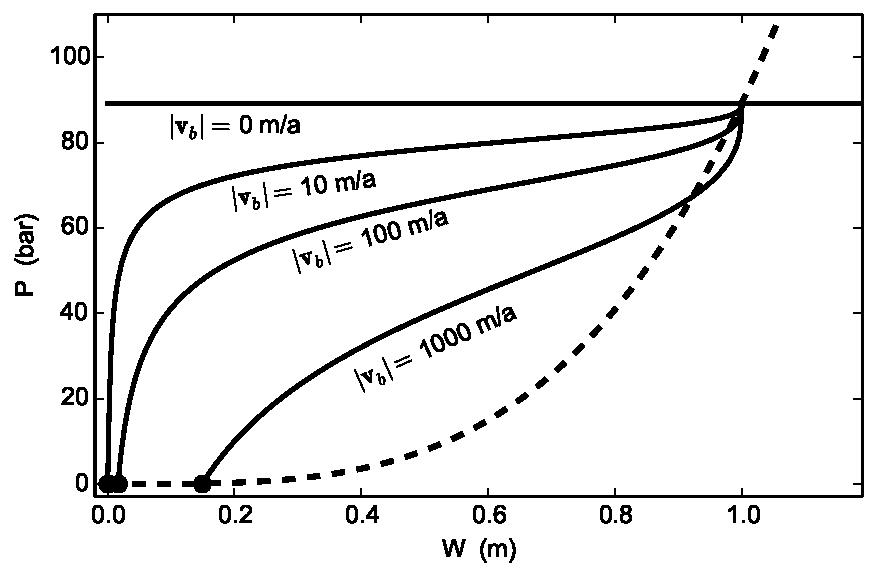
\includegraphics[width=3.0in,keepaspectratio=true]{psteady-vb}
\caption{The steady state function $P(W)$ defined by equation \eqref{eq:PofWsteady} depends on the sliding speed $|\bv_b|$.  Four cases are shown.  All use $W_r=1$ m and a uniform ice thickness of $H=1000$ m.  Values of $W_c$ are indicated by black dots at $P=0$.  Relation \eqref{eq:PofWFC} (dashed black) is shown with $W_{\text{crit}}=1$ m for comparison.}
\label{fig:psteady-vb}
\end{figure}

\begin{figure}[ht]
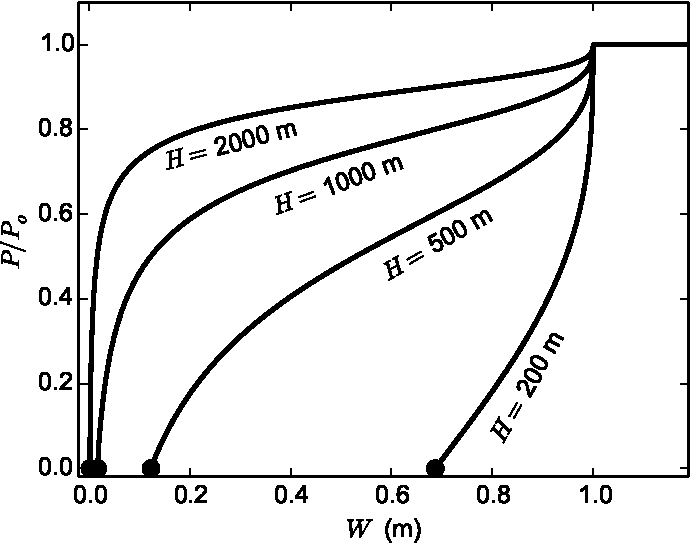
\includegraphics[width=3.0in,keepaspectratio=true]{psteady-Po}
\caption{The graph of $P(W)$ defined by \eqref{eq:PofWsteady} also depends on overburden pressure $P_o=\rho_i g H$.  We fix $|\bv_b|=100$ m/a and $W_r=1$ m and consider four cases of uniform thickness $H$.}
\label{fig:psteady-Po}
\end{figure}

Recall that \cite{FlowersClarke2002_theory} propose function $P_{FC}(W)$ for both steady and nonsteady circumstances.  Both functions $P(W)$ in \eqref{eq:PofWsteady} and $P_{FC}(W)$ in \eqref{eq:PofWFC} are increasing.  They both relate the water pressure to the overburden pressure $P_o$.  However, while in \eqref{eq:PofWsteady} the relation to $P_o$ is additive, in \eqref{eq:PofWFC} it is a multiplicative scaling.  The power law form \eqref{eq:PofWFC} is not justified by the physical reasoning which led to equation \eqref{eq:PofWsteady}, even in steady state.   It would appear that any functional relationship $P(W)$ should also depend on the sliding velocity, as it does here, if cavitation influences the water pressure.  Of course the $W>W_{\text{crit}}$ case gives $P_{FC}(W) > P_o$ in \eqref{eq:PofWFC}, but this condition does not arise in \eqref{eq:PofWsteady}.  In conclusion, an important contrast between the \cite{FlowersClarke2002_theory} theory and the current paper is that we will not assume a relationship $P=P(W)$ in nonsteady conditions, even though such a relation emerges in our theory in the steady state case.

\subsection{Flux in steady state}  We now consider how the steady state water velocity $\bV$, and the associated flux $\bq$, depends on other quantities.  Because $\bV$ depends on $\grad P$, according to equations \eqref{eq:Vsteady} and \eqref{eq:PofWsteady} in steady state we have
\begin{equation}
\frac{\partial P}{\partial W} = \frac{s_b W_r}{3 W^{4/3} (W_r - W)^{2/3}} \label{eq:dPdWsteady}
\end{equation}
if $W_c < W < W_r$.  If $W\le W_c$ then $\partial P/\partial W$ is undefined, and if $W>W_r$ then $\partial P/\partial W=0$.  Note that the condition $W_c < W < W_r$ corresponds to the pressure condition $0 < P < P_o$ in steady state.  Formula \eqref{eq:dPdWsteady} and Figures \ref{fig:psteady-vb} and \ref{fig:psteady-Po} agree that $\partial P / \partial W \to \infty$ as $W \upto W_r$.  Equations \eqref{eq:Vsteady}, \eqref{eq:PofWsteady}, and \eqref{eq:dPdWsteady} imply a formula for the velocity in steady state:
\begin{align}
\bV &= - k \bigg[\grad \psi_o - \left(\frac{W_r - W}{W}\right)^{1/3} \grad s_b \label{eq:Vsteadyexpand} \\
    & \qquad \qquad + \frac{s_b W_r}{3 W^{4/3} (W_r - W)^{2/3}} \grad W\bigg], \notag
\end{align}
where $\psi_o = P_o + \rho_w g b$.

Formula \eqref{eq:Vsteadyexpand} helps us understand the steady state meaning of the advective flux ``$\bV W$'' in $\bq=\bV W - D \grad W$.  The direction of water velocity $\bV$ is determined by a combination of a geometric direction ($\grad \psi_o$), a direction derived from spatial variations in the sliding speed ($\grad s_b$), and a diffusive direction ($\grad W$).  Thus a portion of $\bV W$ is diffusive in steady state, in addition to the \emph{a priori} diffusive flux $- D \grad W$.  In fact we can write the flux as a linear combination of gradients,
\begin{equation}
\bq = - k A_1 \grad \psi_o + k A_2 \grad s_b - k A_3 \grad W,  \label{eq:qabstract}
\end{equation}
with coefficients
\begin{align}
&A_1 = W, \label{eq:qcoefficient} \\
&A_2 = \left(W_r - W\right)^{1/3} W^{2/3}, \notag \\
&A_3 = \frac{s_b W_r}{3 (W_r - W)^{2/3} W^{1/3}} + \rho_w g W. \notag
\end{align}
The first two coefficients $A_1,A_2$ go to zero as $W\to 0$, but $A_3$ remains large when $W\to 0$ as long as sliding is occurring ($s_b > 0$).  Thus for low water amount and sustained sliding we should think of the water as diffusing in the layer.  When the water thickness is greater, namely if it is almost the roughness scale ($W\lesssim W_r$), then $A_3$ is large in sliding cases ($s_b>0$); again the effect is diffusive.

Thinking more generally, it is not surprising that when the ice thickness, bed elevation, sliding velocity, or water thickness fields are highly-variable in space then we can expect larger speeds $|\bV|$ in steady state.  The various gradients in formula \eqref{eq:qabstract} reflect this general intuition.  Because the magnitude of the velocity determines the CFL time step restriction \citep{MortonMayers}, large variations in these spatial fields will generally shorten time steps; see section \ref{sec:num}.


\subsection{Hydraulic conductivity in steady state}  Our next observation takes advantage of the above analysis of the flux in steady state: the water amount $W$ roughly scales with $1/k$ where $k$ is the hydraulic conductivity.  In fact, if we combine equation \eqref{eq:masscontsteady} with \eqref{eq:qabstract} and rearrange slightly then we find
\begin{equation}
-\Div \left(A_3 \grad W\right) = \frac{m}{k \rho_w} + \Div \left(A_1 \grad \psi_o\right) - \Div \left(A_2 \grad s_b\right).  \label{eq:ellipticforWsteadyone}
\end{equation}
One may regard \eqref{eq:ellipticforWsteadyone} as a non-linear elliptic equation for $W$.  In fact, in the case where $H$, $b$, and $|\bv_b|$ are all spatially-uniform, so that $\grad \psi_o = \grad s_b = 0$, equation \eqref{eq:ellipticforWsteadyone} is of the form $-\Div \left(A_3(W) \grad W\right) = m/(k \rho_w)$ where $A_3(W) = A_3$ is given in \eqref{eq:qcoefficient}.  If $W$ is both bounded away from zero and bounded away from the roughness scale $W_r$ (i.e.~there is $\eps>0$ so that $\eps < W < W_r-\eps$) then this equation is uniformly elliptic.  Thus a maximum principle applies \citep{Evans}.  This means that if there is a nonnegative basal melt rate in any region then the maximum of $W$ will equal or exceed the maximum of $W$ along the boundary of that region, so the graph of $W$ is concave down.  However, if $W\approx 0$  or $W\lesssim W_r$ then the diffusivity coefficient $A_3(W)$ will be large and so the values of $W$ away from the boundary will be flattened-out by the resulting fast diffusion.

Furthermore the values of $W$ will scale with $1/k$.  Indeed, for the simpler equation $-\Div \left(D_0 \grad W\right) = m_0/(k \rho_w)$, with $D_0,m_0$ positive constants, on a disc of radius $L$, and zero boundary values, the solution $W(r) = m_0 (1-(r/L)^2) / (4 k D_0 \rho_w)$ has a maximum value $W(0)$ which precisely scales as $1/k$.  As seen in numerical results, the solution $W$ of \eqref{eq:ellipticforWsteadyone} will also scale with $1/k$ if $\grad \psi_o$ and $\grad s_b$ are not too large, though fast-diffusion flattening of the maximum of $W$ will occur when $W$ is close to the limits of the interval $[0,W_r]$.


\section{An exact steady state solution}  \label{sec:exactsolution}

\subsection{Radial equations}  The above steady equations are the basis on which we now build a nearly-exact solution for $W$ and $P$ in the map-plane, in a case with nontrivial overburden pressure and nontrivial ice sliding speed.  This solution, which is useful for verifying numerical schemes, depends on the numerical solution of a scalar first-order ODE initial value problem, something we can do with high accuracy.  Traveling wave exact solutions in one horizontal dimension appear in \cite{Schoofetal2012}.

Consider steady state equations \eqref{eq:Vsteady}--\eqref{eq:masscontsteady}, and assume all quantities only depend on the radial coordinate $r = \sqrt{x^2+y^2}$.  One may eliminate $\bV$.  In the flat bed case ($b=0$) the resulting pair of equations is
\begin{align}
&q = - k W\, \left(\frac{dP}{dr} + \rho_w g \frac{dW}{dr}\right), \label{eq:rsflux} \\
&\frac{1}{r}\frac{d}{dr}\left(r\,q\right) = \frac{m}{\rho_w}. \label{eq:rsconserve}
\end{align}

In the case of constant water input where $m = m_0 > 0$, which we assume for the exact solution, we can integrate \eqref{eq:rsconserve} from $0$ to $r$ and use symmetry ($q(0)=0$) to get
\begin{equation}
q(r) = \frac{m_0}{2\rho_w} \, r. \label{eq:qradial}
\end{equation}
Suppose $h(r)$ is given so that $P_o(r)$ is also determined.  Assume that the scaled sliding speed $s_b(r)$ has a bounded derivative and that the solution $W(r)$ satisfies conditions $W_c < W < W_r$; these properties can be verified for the constructed solution.  By combining \eqref{eq:PofWsteady}, \eqref{eq:dPdWsteady}, \eqref{eq:rsflux}, and \eqref{eq:qradial} we can eliminate $q$ and $P$ to find
\begin{align}
&\omega_0\, r = - W\, \bigg[\frac{dP_o}{dr} - \frac{ds_b}{dr} \left(\frac{W_r - W}{W}\right)^{1/3}  \label{eq:ODEfirst} \\
&\qquad \qquad \qquad + \left(\frac{s_b W_r}{3 W^{4/3} (W_r - W)^{2/3}} + \rho_w g\right) \frac{dW}{dr}\bigg] \notag
\end{align}
where $\omega_0 = m_0 / (2 \rho_w k)$.

Equation \eqref{eq:ODEfirst} is a first-order ordinary differential equation (ODE) for $W(r)$.  To put it in the standard form expected by a numerical ODE solver we solve it for $dW/dr$:
\begin{equation}
\frac{dW}{dr} = \frac{\frac{ds_b}{dr} W \tilde W - \Big[\omega_0\, r W^{-1} + \frac{dP_o}{dr}\Big] W^{4/3} \tilde W^{2/3}}{\frac{1}{3} s_b W_r + \rho_w g W^{4/3} \tilde W^{2/3}}.
\label{eq:WradialODE}
\end{equation}
where $\tilde W = W_r - W$ is the amount by which the water is below the roughness scale.

\subsection{A nontrivial solution}  \label{subsect:exactsoln}  Though equation \eqref{eq:WradialODE} has a constant solution $W(r)=W_r$, to generate a nontrivial exact solution we will choose a positive thickness of ice at the margin so that $P_o(L^-)>0$.  Figure \ref{fig:Pexact} shows the solution and this small cliff in particular.  At the ice margin $r=L$ we have water pressure $P=0$ so $W(L)=W_c(L^-)$ is the boundary condition for the ODE.  We assume that at the margin there is some sliding so that $s_b(L^-)>0$, and by \eqref{eq:steadyboundfirst} we require that $s_b(L^-) W_r > P_o(L^-)^3 W(L)$.  The condition at $r=L$ also satisfies $W(L) < W_r$.  Then we integrate \eqref{eq:WradialODE} from $r=L$ to $r=0$.  The central water thickness value $W(0)$ is determined as part of the solution.

It is useful to have an ice cap geometry in which the surface gradient formula is simple so that $dP_o/dr$ in \eqref{eq:WradialODE} is also simple, so we choose a parabolic profile
\begin{equation}
H(r) = H_0 \left(1 - \frac{r^2}{R_0^2} \right) \label{eq:choosebodvardssonh}
\end{equation}
where $H(0)=H_0$ is the height of the center of the ice cap.  It follows that $dP_o/dr = - C r$ where $C=2\rho_i g h_0 R_0^{-2}$.  We choose $L=0.9 R_0$ and we note that $H(L)=0.19 h_0$ is the size of the cliff.

The sliding speed could be determined by a model for stresses at the ice base and within the ice \citep{GreveBlatter2009}, but a coupled ice and water dynamics solution is unnecessary for hydrology model verification.  Instead we choose a well-behaved sliding speed function which has no sliding near the ice cap center, and which increases in the radial direction:
\begin{equation}
|\bv_b|(r) = \begin{cases} 0, & 0 \le r \le R_1, \\
                           v_0  \left(\frac{r-R_1}{L-R_1}\right)^5, & R_1 < r \le L.
             \end{cases}  \label{eq:choosevb}
\end{equation}
It follows from \eqref{eq:definesb} and \eqref{eq:choosevb} that $ds_b/dr$ in \eqref{eq:WradialODE} is bounded and continuous on $0\le r \le L$.

Now we solve ODE \eqref{eq:WradialODE} with initial condition $W(L)$ and using the specific values in Table \ref{tab:verifconstants}.  We use adaptive numerical ODE solvers, both a Runge-Kutta 4(5) Dormand-Prince method and a variable-order stiff solver, with relative tolerance $10^{-12}$ and absolute tolerance $10^{-9}$.  The two solvers gave essentially identical results.  Modest stiffness \citep{AscherPetzold} of ODE \eqref{eq:WradialODE} is observed at $r\approx R_1$.  The result $W(r)$ is shown in Figure \ref{fig:Wexact}.

Because equations \eqref{eq:choosebodvardssonh} and \eqref{eq:choosevb} imply a pressure functional relation $P=P(W,r)$ from \eqref{eq:PofWsteady}, we can also show in Figure \ref{fig:Wexact} the regions of the $r,W$ plane which correspond to overpressure, normal pressure, and underpressure.  We see that $W(r)$ is in the normal pressure region as $r$ decreases from $r=L$ to $r=R_1$, but at $r=R_1$ the function $W(r)$ switches into the overpressure case because there is no sliding.  Figure \ref{fig:Pexact} shows the corresponding pressure solution $P(r)=P(W(r))$ from \eqref{eq:PofWsteady}.

\begin{table*}[ht]
  \centering
  \caption{Constants used in constructing the exact solution.}
  \begin{tabular}{lllp{3.0in}}
    \textbf{Name} & \textbf{Value} & \textbf{Units} & \textbf{Description}\\
\hline
    $\alpha$ & $1$ & & power in flux \\
    $\beta$  & $2$ & & power in flux \\
    $H_0$ & $500$ & m & ice cap center thickness \\
    $k$   & $0.01/(\rho_w g)$ & $\text{m}^3\,\text{s}\,\text{kg}^{-1}$ & hydraulic conductivity \\
    $L$   & $22.5$& km & $=0.9 R_0$; location of cliff \\
    $m_0$ & $0.2\rho_w$ & $\text{kg}\,\text{m}^{-2}\,\text{a}^{-1}$ & constant water input rate; $= 20 \,\text{cm}\,\text{a}^{-1}$ \\
    $R_0$ & $25$  & km & ideal ice cap radius (at which $H\to 0$) \\
    $R_1$ & $5$   & km & radial location $r=R_1$ of onset of sliding \\
    $v_0$ & $100$ & $\text{m}\,\text{a}^{-1}$ & sliding speed scale \\
    $W_r$ & $1$ & m & roughness scale \\
    \hline
  \end{tabular}
 \label{tab:verifconstants}
\end{table*}

\begin{figure}[ht]
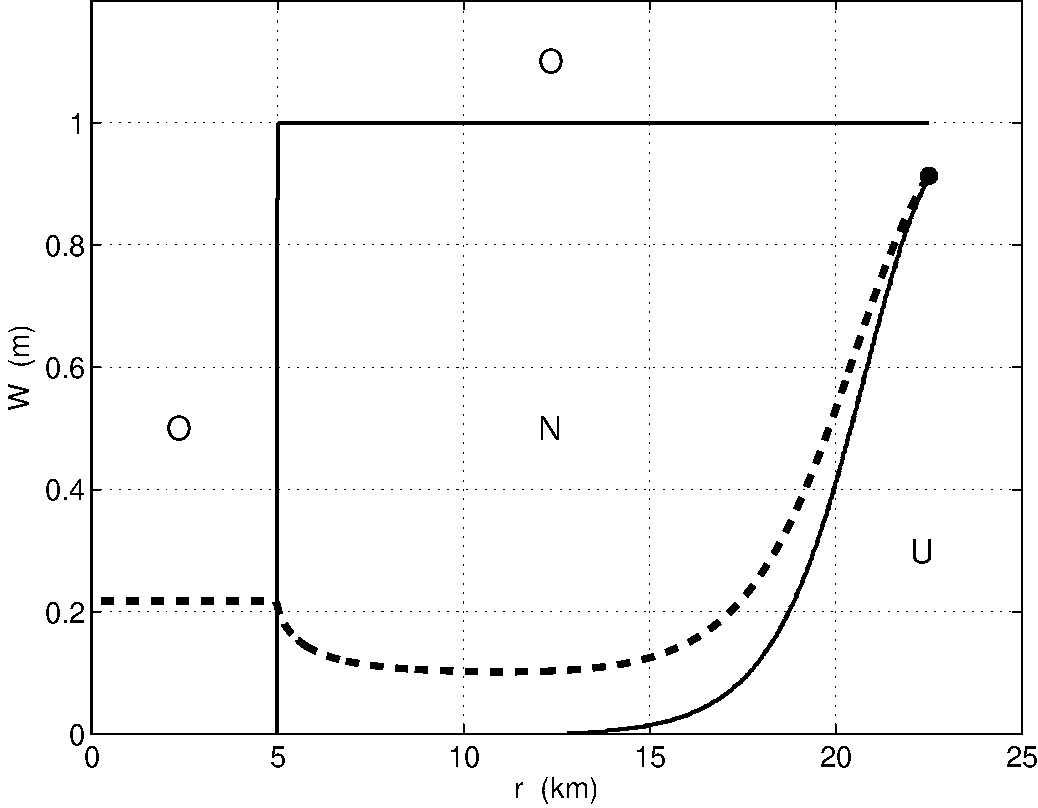
\includegraphics[width=3.0in,keepaspectratio=true]{exact-W-plot-onu}
\caption{An exact radial, steady solution for water thickness $W(r)$ (dashed).  In $r$-versus-$W$ space the overpressure (O), normal pressure (N), and underpressure (U) regions are determined by ice geometry and sliding velocity (solid curves; see text).}
\label{fig:Wexact}
\end{figure}

The reason for stiffness near $R_1$ is that as the sliding goes to zero the cavitation rate goes to zero.  Because creep closure balances cavitation in steady state, effective pressure also goes to zero ($P\to P_o$).  The remaining active mechanisms in the model are the variable overburden pressure and the rate of water input, and they must exactly balance.  In this case \eqref{eq:WradialODE} reduces to the simpler form
\begin{equation}
\frac{dW}{dr} = - \frac{\varphi_o r W^{-1} + \frac{dP_o}{dr}}{\rho_w g}. \label{eq:WradialODEnoslide}
\end{equation}
Though we have not derived it this way, Equation \eqref{eq:WradialODEnoslide} is the steady radial form of the mass conservation equation under the ``$P=P_o$'' closure, namely equation \eqref{eq:PisoverConservation}.

In equation \eqref{eq:WradialODEnoslide} we see that $dW/dr=0$ if $W$ satisfies $W = - \omega_0 r / (dP_o/dr)$.  In our case with geometry \eqref{eq:choosebodvardssonh} this reduces to a constant value $W=W^*= 0.21764$ m because $dP_o/dr$ is linear in $r$.  Both numerical ODE solvers used here confirm that $W(r)$ is asymptotic to this constant value $W^*$ as $r\to 0$, and that $W(r)\approx W^*$ within about 1\% on all of $0\le r \le R_1$.  This is seen in Figure \ref{fig:Wexact}.

\begin{figure}[ht]
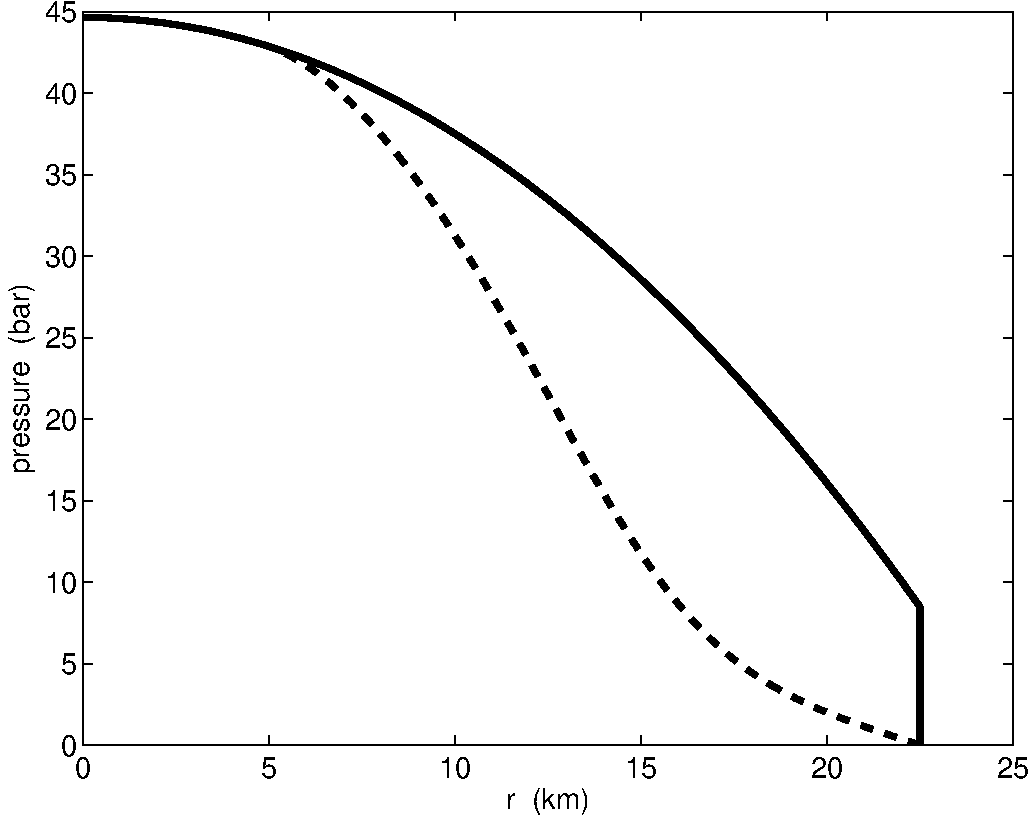
\includegraphics[width=3.0in,keepaspectratio=true]{exact-P-plot}
\caption{An exact radial, steady solution pressure $P(r)$ (dashed) and overburden pressure $P_o$ (solid).}
\label{fig:Pexact}
\end{figure}

In summary, we have derived and analyzed an exact solution, in a case with angular symmetry, of the steady state form of the coupled model \eqref{eq:bluebox}, assuming $\Wtilmax=0$ and $b=0$.  This solution will be helpful in verifying the numerical schemes in the next section.


\section{Numerical schemes}  \label{sec:num}

\subsection{Mass conservation: time-stepping}  Mass conservation equation \eqref{eq:adeqn}, which is part of the combined mathematical model \eqref{eq:bluebox}, will be discretized by an explicit, conservative finite difference method.   A centered, second-order scheme will be applied to the diffusion part.  A pair of schemes for the advection part will be compared, namely first-order upwinding and a higher-order flux-limited upwind-biased method.

We first consider stable time steps.  Stability for the advection schemes occurs with a time step $\Delta t \le \Delta t_{\text{CFL}}$ where
\begin{equation}
\Delta t_{\text{CFL}} \left(\frac{\max |u|}{\Delta x} + \frac{\max |v|}{\Delta y}\right) = \frac{1}{2}. \label{eq:dtCFL}
\end{equation}
Because of the additional diffusion process, for stability the time step should also satisfy $\Delta t \le \Delta t_{W}$  where \citep{MortonMayers}
\begin{equation}
\Delta t_W\, 2 \max D \left(\frac{1}{\Delta x^2} + \frac{1}{\Delta y^2}\right) = \frac{1}{2}. \label{eq:dtDIFFW}
\end{equation}
The condition $\Delta t \le \min\{\Delta t_{\text{CFL}}, \Delta t_W\}$ is sufficient for stability and convergence of the scheme for \eqref{eq:adeqn}.  Below we show this for the first-order upwind scheme, but standard theory suggests the same conclusion for the higher-order flux-limited advection scheme \citep{HundsdorferVerwer2010}.

We can understand the scale of these restrictions better by considering an example using the parameter values in Table \ref{tab:constants}.  We ran the model on a $\Delta x = \Delta y = 250$ m grid to approximate steady state for the subglacial hydrology of \Nbreen \citep{vanPeltthesis,vanPeltetal}, using observed ice and bedrock geometry, a hypothesized water input distribution with average value about 1 m $\text{a}^{-1}$, and a glacier-wide constant sliding rate of $50$ m $\text{a}^{-1}$.  The result is that the maximum computed water speed $|\bV|$ is about $0.2$ m $\text{s}^{-1}$ so the advective restriction \eqref{eq:dtCFL} is $\Delta t_{\text{CFL}} \approx 300\,\text{s} \approx 10^{-5}\,\text{a}$.  Computed diffusivity $D = \rho_w g K W$ has a maximum value that varies significantly in time, $0.1 \le \max D \le 5 \,\text{m}^2\,\text{s}^{-1}$.  Diffusive restriction \eqref{eq:dtDIFFW} using value $\max D=1\,\text{m}^2\,\text{s}^{-1}$ is $\Delta t_W \approx 8000\,\text{s} \approx 2.5 \times 10^{-4}\,\text{a}$.  Thus in this simulation $\Delta t_W \approx 25 \Delta t_{CFL}$.

This example suggests that, unless both the global peak velocity is unusually slow, and deep subglacial lakes develop so that $D$ is large, the diffusive time scale is significantly longer than the CFL time scale for a $250$ m grid.  The scaling $\Delta t_W = O(\Delta x^2)$ versus $\Delta t_{CFL} = O(\Delta x^1)$ makes it clear that under sufficient spatial grid refinement $\Delta t_W$ is the controlling restriction, but we suppose that $\Delta t_{CFL}$ is controlling for $\Delta x \gg 100$ m.  We will see below, however, that the time step restriction associated to an explicit time-stepping method for the pressure equation is typically shorter than either of $\Delta t_W,\Delta t_{CFL}$, and it scales as $O(\Delta x^2)$ like $\Delta t_W$.  If implicit time-stepping is used for the pressure equation, which requires variational inequality treatment \citep{Schoofetal2012}, then the time scales $\Delta t_W, \Delta t_{CFL}$ addressed here are the only restrictions.  The time step restriction $\Delta t_W$ could be removed by implicit steps for the mass-conservation equation, though it would seem this requires another variational inequality formulation because of the lower bound $W\ge 0$.  Our observation that $\Delta t_{CFL} \ll \Delta t_W$ for practical ice sheet grids suggests that implicit time-stepping for the mass-conservation equation is not beneficial.

\begin{figure}[ht]
\centering
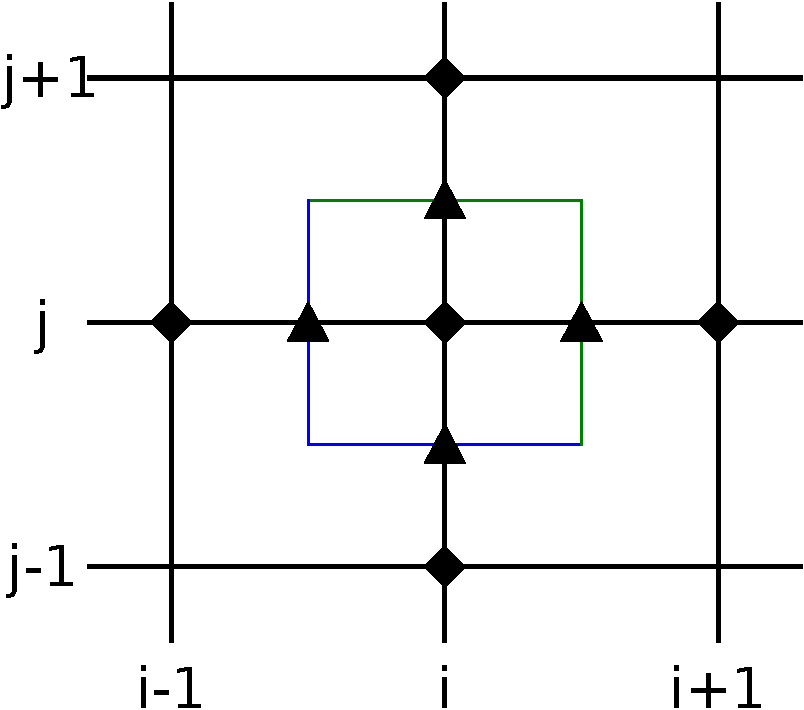
\includegraphics[width=2.2in,keepaspectratio=true]{diffstencil}
\bigskip
\caption{Numerical schemes \eqref{eq:Wfd} and \eqref{eq:Pfd} use a grid-point-centered cell.  Velocities, diffusivities, and fluxes are evaluated at staggered grid locations (triangles at centers of cell edges denoted $e,w,n,s$).  State functions $W,P$ are located at regular grid points (diamonds).}
\label{fig:stencil}
\end{figure}

\subsection{Mass conservation: spatial discretization}  To set notation, suppose the rectangular computational domain has $M_x \times M_y$ gridpoints $(x_i,y_j)$ with uniform spacing $\Delta x,\Delta y$.  Let $\Wlij \approx W(t_l,x_i,y_j)$, $(\Wtil)_{ij}^l \approx \Wtil(t_l,x_i,y_j)$, and $\Plij \approx P(t_l,x_i,y_j)$ denote the numerical approximations.

We will compute velocity components and flux components at the staggered (cell-face-centered) points shown in Figure \ref{fig:stencil} using centered finite difference approximations of equations \eqref{eq:vexpression} and \eqref{eq:qexpression}.  We use ``compass'' indices such as $u_e = u_{i+1/2,j}$ for the ``east'' staggered value of $u$ and $v_n = v_{i,j+1/2}$ for the ``north'' staggered value of $v$.  Similarly we use compass indices for staggered grid values of the water layer thickness, computed by averaging regular grid values:
\begin{align}
W_e &= (W_{i,j}^l + W_{i+1,j}^l)/2, \label{eq:stagW} \\
W_n &= (W_{i,j}^l + W_{i,j+1}^l)/2. \notag
\end{align}

The nonlinear effective conductivity $K$ from \eqref{eq:Kdefine} is also needed at staggered locations.  As a notational convenience define $R=P+\rho_w g b$ and define these staggered-grid values \citep[compare][]{Mahaffy}:
\begin{align*}
&\Pi_e = \left|\frac{R_{i+1,j}-R_{i,j}}{\Delta x}\right|^2 \\
&\qquad \qquad + \left|\frac{R_{i+1,j+1}+R_{i,j+1} - R_{i+1,j-1}-R_{i,j-1}}{4\Delta y}\right|^2, \\
&\Pi_n = \left|\frac{R_{i+1,j+1}+R_{i+1,j} - R_{i-1,j+1}-R_{i-1,j}}{4\Delta x}\right|^2 \\
&\qquad \qquad + \left|\frac{R_{i,j+1}-R_{i,j}}{\Delta y}\right|^2.
\end{align*}
Thereby define
\begin{equation}
K_e = k W_e^{\alpha-1} \Pi_e^{(\beta-2)/2}, \quad K_n = k W_n^{\alpha-1} \Pi_n^{(\beta-2)/2}.  \label{eq:stagK}
\end{equation}
The velocity components are then found by differencing:
\begin{align}
u_e &= - K_e \left(\frac{P_{i+1,j}-P_{i,j}}{\Delta x} + \rho_w g \frac{b_{i+1,j}-b_{i,j}}{\Delta x}\right),  \label{eq:velocitycomp} \\
v_n &= - K_n \left(\frac{P_{i,j+1}-P_{i,j}}{\Delta y} + \rho_w g \frac{b_{i,j+1}-b_{i,j}}{\Delta y}\right). \notag
\end{align}
Similarly for diffusivity we have
\begin{equation}
D_e = \rho_w g K_e W_e, \qquad D_n = \rho_w g K_n W_n.  \label{eq:diffusivitycomp}
\end{equation}
We get the remaining staggered-grid quantities by shifting indices:
\begin{align*}
u_w &= u_e\big|_{(i-1,j)}, \quad K_w = K_e\big|_{(i-1,j)}, \quad D_w = D_e\big|_{(i-1,j)}, \\
v_s &= v_n\big|_{(i,j-1)}, \quad K_s = K_n\big|_{(i,j-1)}, \quad D_s = D_n\big|_{(i,j-1)}.
\end{align*}

Now we define $Q_e(u_e)$, $Q_w(u_w)$, $Q_n(v_n)$, and $Q_s(v_s)$ as the face-centered (staggered-grid) normal components of the advective flux $\bV W$.  These quantities are described in more detail in the next subsection.  They use only the staggered velocity component but there is upwinding to determine which $W$ value, or combination of $W$ values, is used.

The grid values of $\Div \bq = \Div (\bV W) - \Div (D \grad W)$ using \eqref{eq:velocitycomp} and \eqref{eq:diffusivitycomp} now become:
\begin{align}
&\mathcal{D}_{i,j} =  \frac{Q_e(u_e) - Q_w(u_w)}{\Delta x} + \frac{Q_n(v_n) - Q_s(v_s)}{\Delta y}  \label{eq:fluxdivgrid} \\
&\qquad \qquad - \frac{D_e (W_{i+1,j}^l - \Wlij) - D_w (\Wlij - W_{i-1,j}^l)}{\Delta x^2} \notag \\
&\qquad \qquad - \frac{D_n (W_{i,j+1}^l - \Wlij) - D_s (\Wlij - W_{i,j-1}^l)}{\Delta y^2},  \notag
\end{align}
where ``$\mathcal{D}$'' is for ``divergence.''  To ensure conservation, $Q_e(u_e)$ used in computing $\mathcal{D}_{i,j}$ must be the same as $Q_w(u_w)$ used in computing $\mathcal{D}_{i+1,j}$, and similarly for ``north'' and ``south'' staggered fluxes; our formulas have these properties.

Now our scheme for approximating mass conservation equation \eqref{eq:adeqn} is
\begin{equation}
\frac{W_{i,j}^{l+1} - W_{i,j}^l}{\Delta t} + \frac{(\Wtil)_{i,j}^{l+1} - (\Wtil)_{i,j}^l}{\Delta t} = - \mathcal{D}_{i,j} + \frac{m_{ij}}{\rho_w}.    \label{eq:Wfd}
\end{equation}
The updated value of $\Wtil$, which appears on the left side of \eqref{eq:Wfd}, is computed by trivial integration of equation \eqref{eq:tilldynamics}, namely
\begin{equation}
(\Wtil)_{i,j}^{l+1} = (\Wtil)_{i,j}^l + \Delta t \left(\frac{m_{ij}}{\rho_w} - C_d\right).  \label{eq:tillupdatefd}
\end{equation}
The right-hand-side value is used if it is in the closed interval $[0,\Wtilmax]$, but otherwise the bounds $0\le \Wtil \le \Wtilmax$ are enforced.  Once $\Wtil^{l+1}$ is computed, the value of $W^{l+1}$ can be updated by \eqref{eq:Wfd} in a mass-conserving way.

Assuming no error in the flux components $Q$, the local truncation error \citep{MortonMayers} of scheme \eqref{eq:Wfd} would be $O(\Delta t^1 + \Delta x^2 + \Delta y^2)$ as an approximation of \eqref{eq:adeqn}.  The actual truncation error depends on the nature of the approximation which generates the discrete fluxes; see subsection \ref{subsect:discretefluxes} below.

\subsection{Discrete advective fluxes}  \label{subsect:discretefluxes}  Well-chosen discrete approximations of the advective flux $\bV W$ are important to the accuracy of the whole scheme.  Mass conservation of these schemes essentially follows from using the staggered-grid values as described in the last subsection.  In our explicit time-stepping framework we expect, and can show in the simpler first-order case (see next subsection), that stability follows from enforcing a CFL restriction.  To examine accuracy, however, we test two flux discretization schemes \eqref{eq:Wfd}, namely first-order upwind and the Koren flux-limited third-order scheme \citep{HundsdorferVerwer2010}.  Both schemes achieve non-oscillation and positivity, but with different local truncation error and complexity of implementation.  The third-order scheme is best explained as a modification of the better-known conservative (``donor cell''; \cite{LeVeque}) first-order upwind scheme we use.

In fact, the following formulas apply in the cases $u_e \ge 0$, $u_e < 0$, $v_n \ge 0$, and $v_n < 0$, respectively:
\begin{align}
&Q_e(u_e) = u_e \left[W_{i,j} + \Psi(\theta_{i}) (W_{i+1,j} - W_{i,j})\right], \label{eq:adfluxes} \\ 
&Q_e(u_e) = u_e \left[W_{i+1,j} + \Psi\left((\theta_{i+1})^{-1}\right) (W_{i,j} - W_{i+1,j})\right],  \notag \\
&Q_n(v_n) = v_n \left[W_{i,j} + \Psi(\theta_{j}) (W_{i,j+1} - W_{i,j})\right], \notag \\
&Q_n(v_n) = v_n \left[W_{i,j+1} + \Psi\left((\theta_{j+1})^{-1}\right) (W_{i,j} - W_{i,j+1})\right].\notag
\end{align}
The subscripted $\theta$ quotients are as follows:
\begin{align*}
\theta_i &= \frac{W_{i,j}-W_{i-1,j}}{W_{i+1,j} - W_{i,j}}, & (\theta_{i+1})^{-1} &= \frac{W_{i+2,j}-W_{i+1,j}}{W_{i+1,j} - W_{i,j}}, \\
\theta_j &= \frac{W_{i,j}-W_{i,j-1}}{W_{i,j+1} - W_{i,j}}, & (\theta_{j+1})^{-1} &= \frac{W_{i,j+2}-W_{i,j+1}}{W_{i,j+1} - W_{i,j}}.
\end{align*}
The first-order upwind scheme simply sets $\Psi(\theta)=0$ in formulas \eqref{eq:adfluxes}.  The Koren scheme ``limits'' its third-order and positive-coefficient correction to the upwind scheme by using this formula \citep{HundsdorferVerwer2010}:
\begin{equation}
\Psi(\theta) = \max\left\{0,\min\Big\{1,\theta,\frac{1}{3}+\frac{1}{6} \theta\Big\}\right\}.  \label{eq:korenPsi}
\end{equation}
Thus one does not compute $\theta$ quotients at all when using first-order upwind.  On the other hand, when using the Koren flux-limiter the stencil in Figure \ref{fig:stencil} is extended because regular grid neighbors $W_{i+2,j}$, $W_{i-2,j}$, $W_{i,j+2}$, $W_{i,j-2}$ are also involved in updating $W_{i,j}$.

The flux-correction-limited Koren third-order scheme bypasses the first-order limitation of positive linear finite difference/volume schemes imposed by Godunov's barrier theorem \citep[section I.7.1]{HundsdorferVerwer2010} by having a nonlinear correction formula, i.e. the combination of \eqref{eq:adfluxes} and \eqref{eq:korenPsi} above.  Though the Koren scheme is usually third-order where smoothness allows, it reverts to first-order at extrema and other non-smooth areas where $\theta \gg 1$ or $\theta \ll 1$.

For either the first-order or Koren schemes, if the water input $m$ is negative then we must actively enforce the positivity of the water thickness $W$.  Positivity of the source-free advection-diffusion scheme is a desirable property but it does not ensure positivity of the solution if there is actual water removal (i.e.~if $(m/\rho_w) - \partial \Wtil/\partial t < 0$).  Therefore we project (reset) $W$ to be nonnegative at the end of each time step.

\subsection{Mass conservation: positivity and stability}  Explicit numerical scheme \eqref{eq:Wfd} for the mass conservation PDE \eqref{eq:adeqn}, combined with the first-order upwind case of formulas \eqref{eq:adfluxes}, is sufficiently simple so that we can analyze its stability properties.  For this scheme we now sketch a maximum principle argument which shows stability \citep{MortonMayers}.  The argument also shows positivity \citep{HundsdorferVerwer2010} as long as the total water input is nonnegative, but here only the case $m = 0$ and $\Wtilmax=0$ case is shown.  Also we consider only the upwinding case where the discrete velocities at cell interfaces are nonnegative: $u_e\ge 0$, $u_w\ge 0$, $v_n\ge 0$, $v_s\ge 0$.  The other upwinding cases can be handled by similar arguments.

Define $\nu_x = \Delta t/\Delta x$, $\nu_y = \Delta t/\Delta y$, $\mu_x = \Delta t/\Delta x^2$, and $\mu_y = \Delta t/\Delta y^2$.  Collecting terms in \eqref{eq:Wfd} to write the new value as a linear combination of the old values, we get
\begin{align}
 W_{i,j}^{l+1} &= (\nu_x u_w + \mu_x D_w) W_{i-1,j}^l + (\mu_x D_e) W_{i+1,j}^l \notag \\
      &\qquad + (\nu_y v_s + \mu_y D_s) W_{i,j-1}^l + (\mu_y D_n) W_{i,j+1}^l  \notag \\
      &\qquad + \Big[1 - \nu_x u_e - \nu_y v_n \notag \\
      &\qquad\qquad - \mu_x (D_e + D_w) - \mu_y (D_n + D_s)\Big] \Wlij \notag \\
  &= \tilde A\, W_{i-1,j}^l + \tilde B\, W_{i+1,j}^l + \tilde C\, W_{i,j-1}^l \notag \\
  &\qquad + \tilde D\, W_{i,j+1}^l + \tilde E\, \Wlij. \label{eq:lincomb}
\end{align}
Because of our assumption about nonnegative velocities, and noting that the diffusivities are nonnegative, we see that coefficients $\tilde A,\tilde B,\tilde C,\tilde D$ are all nonnegative.  Only $\tilde E$ could be negative, depending on values of $\nu_x, \nu_y, \mu_x$, and $\mu_y$.  

Requiring $\tilde E$ in \eqref{eq:lincomb} to be nonnegative is a sufficient stability condition \citep{MortonMayers}, which we generate based on an equal split between advective and diffusive parts.  First there is a CFL restriction for the advection terms, namely $\nu_x \alpha_e + \nu_y \beta_n \le \frac{1}{2}$, which is condition \eqref{eq:dtCFL} when generalized to all upwinding cases.  The second is a time-step restriction on the diffusion, namely $\mu_x (D_e + D_w) + \mu_y (D_n + D_s) \le \frac{1}{2}$, which is condition \eqref{eq:dtDIFFW}.  If both \eqref{eq:dtCFL} and \eqref{eq:dtDIFFW} hold then the coefficient $\tilde E$ in \eqref{eq:lincomb} is nonnegative.

Because the coefficients in linear combination \eqref{eq:lincomb} also add to one, as the reader may check, it follows  from \eqref{eq:dtCFL} and \eqref{eq:dtDIFFW} that the scheme is stable \citep{MortonMayers}.  It also follows from \eqref{eq:dtCFL} and \eqref{eq:dtDIFFW} that if $\Wlij\ge 0$ for all $i,j$ then \eqref{eq:lincomb} gives $W_{ij}^{l+1}\ge 0$, in this $m=0$ and $\Wtilmax=0$ case, which is our positivity claim.  Thus, under conditions \eqref{eq:dtCFL} and \eqref{eq:dtDIFFW}, scheme \eqref{eq:Wfd} is stable and positivity-preserving.

\subsection{Discretization of the pressure equation}  The pressure evolution equation \eqref{eq:regpressureequation} is a nonlinear diffusion with additional ``reaction'' terms associated to opening and closing.  The time step restriction for our explicit pressure scheme is comparable to \eqref{eq:dtDIFFW}, though the proof above for the stability of the mass conservation scheme does not suffice to \emph{prove} stability.  That is, if the time step satisfies $\Delta t \le \Delta t_P$, where
\begin{equation}
\Delta t_P\, \left(\frac{2 \max D}{\phi_0}\right) \left(\frac{1}{\Delta x^2} + \frac{1}{\Delta y^2}\right) = 1 \label{eq:dtDIFFP}
\end{equation}
then we assert that, and observe in practice that, the scheme is stable.  From \eqref{eq:dtDIFFW} the resulting time step $\Delta t_P$ is a fraction of $\Delta t_W$:
\begin{equation}
\Delta t_P = 2 \phi_0\, \Delta t_W.  \label{eq:dtDIFFPfromW}
\end{equation}

We can again be quantitative in a particular example.  Consider the same 250 m simulation of the hydrology of \Nbreen as earlier.  With $\phi_0 = 0.01$ we have $\Delta t_P$ which is 50 times smaller than $\Delta t_W$ and half of $\Delta t_{\text{CFL}}$:
\begin{align*}
  &\Delta t_W            \approx 8000 \text{ s} &&\text{ from \eqref{eq:dtDIFFW}}, \\
  &\Delta t_{\text{CFL}} \approx 300  \text{ s} &&\text{ from \eqref{eq:dtCFL}}, \\
  &\Delta t_P            \approx 160  \text{ s} &&\text{ from \eqref{eq:dtDIFFPfromW}.}
\end{align*}
This analysis suggests that the numerical scheme for pressure diffusion, given next, may often have the shortest time step, but it may be comparable to CFL.  Note that $\Delta t_{\text{CFL}}=O(\Delta x)$ while $\Delta t_W$ and $\Delta t_P$ are $O(\Delta x^2)$.  The time step restriction $\Delta t_P$ scales with the adjustable regularizing porosity $\phi_0$ so we can make it more or less severe.

The scheme we use for the pressure equation \eqref{eq:regpressureequation} is similar to the scheme we have just presented for the mass continuity equation \eqref{eq:adeqn}.  Denote $\psi_{i,j}^l = P_{i,j}^l + \rho_w g (b_{i,j}^l + W_{i,j}^l)$.  Let $\mathcal{O}_{ij} = c_1 |\bv_b|_{i,j} \left(W_r - \Wlij\right)_+$ and $\mathcal{C}_{ij} = c_2 A \left(\rho_i g H_{i,j} - \Plij\right)^3 \Wlij$ be the gridded values of the cavitation-opening and creep-closure rates.  Also define the sum of all zero order (i.e.~without spatial derivatives) terms
\begin{equation}
Z_{ij} = \mathcal{C}_{ij} - \mathcal{O}_{ij} + \frac{m_{ij}}{\rho_w} - \frac{(\Wtil)_{ij}^{l+1} - (\Wtil)_{ij}^l}{\Delta t}.  \label{eq:defnZ}
\end{equation}
Using \eqref{eq:fluxdivgrid} for the flux divergence, the scheme for pressure equation \eqref{eq:regpressureequation} is now
\begin{equation}
\frac{\phi_0}{\rho_w g} \frac{P_{i,j}^{l+1} - \Plij}{\Delta t} = - \mathcal{D}_{i,j} + Z_{ij},  \label{eq:Pfd}
\end{equation}
or, in explicit update form,
\begin{equation}
P_{i,j}^{l+1} = \Plij + \frac{\rho_w g\,\Delta t}{\phi_0} \left(- \mathcal{D}_{i,j} + Z_{ij}\right). \label{eq:Pfdupdate}
\end{equation}
Because equation \eqref{eq:defnZ} uses the updated value $(\Wtil)_{ij}^{l+1}$, equation \eqref{eq:tillupdatefd} must be applied before \eqref{eq:Pfdupdate} can be used to update $P$ to the new time $t_{l+1}$.

There are special cases at the boundaries of the active subglacial layer: (\emph{i}) where there is no ice $H_{i,j}=0$ and land ($b_{i,j}>0$) we set $P_{i,j}^{l+1}=0$, (\emph{ii}) where the ice is floating we set $P_{i,j}^{l+1}=(P_o)_{i,j}$, and (\emph{iii}) where there is grounded ice ($H_{i,j}>0$) and no water ($W_{i,j}^l=0$) we set $P_{i,j}^{l+1}=(P_o)_{i,j}$ if there is no basal sliding and $P_{i,j}^{l+1}=0$ if there is sliding (because of cavitation; see equation \eqref{eq:PofWsteady}).

\subsection{One time step of the model}  Mathematical model \eqref{eq:bluebox} evolves $W$, $\Wtil$, and $P$.  Here we describe one time step of the fully-discretized evolution.  For convenience we treat the ice and bedrock geometry, and the ice sliding speed, as fixed, and so $h_{i,j}$, $b_{i,j}$, $(P_o)_{i,j}$, and $|\bv_b|_{i,j}$ are all denoted as time-independent.

The ice geometry may be quite general, with ice-free land or floating ice allowed at any location $(x_i,y_j)$.  The ice geometry determines boolean ``masks'' for grid cell state (based on zero sea level elevation):
\begin{align*}
\text{\texttt{icefree}}_{i,j} &= (h_{i,j} > 0)\, \&\, (h_{i,j} = b_{i,j}), \\
\text{\texttt{float}}_{i,j}   &= (\rho_i (H_{\text{float}})_{i,j} < - \rho_{sw}\, b_{i,j}).
\end{align*}
Here we take a sea-water density $\rho_{sw}=1028.0$ and $H_{\text{float}}=h_{i,j} / (1 - r)$  is the thickness of the ice if it is floating, where $r=\rho_i / \rho_{sw}$.  Note that $\text{\texttt{float}}_{i,j}$ is also true in ice-free ocean.  The subglacial hydrology model exists only for grounded ice, that is, only if both \texttt{icefree} and \texttt{float} are false.  The other mask cases provide boundary conditions when they are neighbors to grounded ice-filled cells.

One time step follows this algorithm:

\renewcommand{\labelenumi}{\emph{(\roman{enumi})}}
\begin{enumerate}
\item Start with values $\Wlij$, $(\Wtil)_{i,j}^l$, $\Plij$ which satisfy the bounds $W\ge 0$, $0\le \Wtil \le \Wtilmax$, and $0 \le P \le P_o$.
\item Get $(\Wtil)_{i,j}^{l+1}$ by \eqref{eq:tillupdatefd}.  If $\text{\texttt{icefree}}_{i,j}$ or $\text{\texttt{float}}_{i,j}$ then set $(\Wtil)_{i,j}^{l+1}=0$.
\item Get $W$ values averaged onto the staggered grid from \eqref{eq:stagW}, staggered grid values of the effective conductivity $K$ from \eqref{eq:stagK}, velocity components $u$, $v$ at staggered grid locations from \eqref{eq:velocitycomp}, and staggered grid values of the diffusivity $D$ from \eqref{eq:diffusivitycomp}.
\item Get time step $\Delta t = \min\{\Delta t_{\text{CFL}}, \Delta t_W, \Delta t_P\}$ using criteria \eqref{eq:dtCFL}, \eqref{eq:dtDIFFW}, and \eqref{eq:dtDIFFPfromW}, based on the current staggered-grid values of $u,v,$ and $D$.
\item Using \eqref{eq:adfluxes} and a particular flux-limiter, compute the advective fluxes $Q_e(\alpha_e)$ at all staggered-grid points $(i+1/2,j)$ and $Q_n(\beta_n)$ at all staggered-grid points $(i,j+1/2)$.
\item Get approximations $\mathcal{D}_{i,j}$ of the flux divergence from \eqref{eq:fluxdivgrid}.  For each direction (i.e.~$x$- and $y$-directions), do not compute the divided-difference contribution to the flux divergence in \eqref{eq:fluxdivgrid} if either neighbor is \texttt{icefree} or \texttt{float}.
\item If $\text{\texttt{icefree}}_{i,j}$ then set $P_{i,j}^{l+1}=0$.  If $\text{\texttt{float}}_{i,j}$ then set $P_{i,j}^{l+1} = (P_o)_{i,j}$.  If $\Wlij=0$ and $\text{\texttt{icefree}}_{i,j}$ and $\text{\texttt{float}}_{i,j}$ are both false, then set $P_{i,j}^{l+1} = (P_o)_{i,j}$.  Then use \eqref{eq:Pfdupdate} to compute values for $P_{i,j}^{l+1}$ at the remaining locations.
\item If $P_{i,j}^{l+1}$ does not satisfy bounds $0 \le P \le P_o$ then reset (project) into this range.
\item If $\text{\texttt{icefree}}_{i,j}$ or $\text{\texttt{float}}_{i,j}$ then set $W_{i,j}^{l+1}=0$.  Otherwise use \eqref{eq:Wfd} to compute values for $W_{i,j}^{l+1}$.
\item If $W_{i,j}^{l+1}<0$ then reset (project) $W_{i,j}^{l+1}=0$.
\item Update time $t_{l+1}=t_l+\Delta t$ and repeat at \emph{(i)}.
\end{enumerate}

\medskip
This recipe goes with a reporting scheme for mass conservation.  Note that in steps \emph{(ii)} and \emph{(ix)} water is lost or gained at the margin where either the ice thickness goes to zero on land (margins), or at locations where the ice becomes floating (grounding lines).  Because such loss/gain may be the modeling goal---users want hydrological discharge---these amounts are reported.  This reporting scheme also tracks the projections in step \emph{(x)}, which represent a mass conservation error which goes to zero under the continuum limit $\Delta t\to 0$.


\section{PISM options for hydrology models} \label{sec:pismdoc}

In this section we document the runtime options for the PISM hydrology model \citep{pism-user-manual}.  There are three choices of model equations, namely \texttt{distributed}, \texttt{routing}, and \texttt{null}.  The first of these is the complete model described in this paper.  The other two are reductions; we list them in order of decreasing complexity.  We also give a concordance between the symbols in this paper and the relevant PISM configuration parameters.

\begin{table*}[t]
  \caption{Correspondence between symbols in this paper and PISM configuration parameter names.  Alphabetical by parameter name.  All of these are used in the \texttt{distributed} model, with the indicated subsets also used in the \texttt{routing} and \texttt{null} models.} \vskip4mm \centering
  \begin{tabular}{llcc} \tophline
    \textbf{PISM configuration name} & \textbf{Symbol} & \textbf{\texttt{routing}} & \textbf{\texttt{null}} \\
    \middlehline
    \verb|fresh_water_density| & $\rho_w$ & $\times$ & $\times$ \\
    \verb|hydrology_cavitation_opening_coefficient| & $c_1$ \\
    \verb|hydrology_creep_closure_coefficient| & $c_2$ \\
    \verb|hydrology_gradient_power_in_flux| &  $\beta$ & $\times$ & \\
    \verb|hydrology_hydraulic_conductivity| & $k$ & $\times$ & \\
    \verb|hydrology_regularizing_porosity| & $\phi_0$ \\
    \verb|hydrology_roughness_scale| & $W_r$ \\
    \verb|hydrology_thickness_power_in_flux| &  $\alpha$ & $\times$ & \\
    \verb|hydrology_tillwat_decay_rate| & $C_d$ & $\times$ & $\times$ \\
    \verb|hydrology_tillwat_max| & $\Wtilmax$ & $\times$ & $\times$ \\
    \verb|ice_density| & $\rho_i$ & $\times$ & $\times$ \\
    \verb|ice_softness| & $A$ \\
    \verb|standard_gravity| & $g$ & $\times$ & $\times$ \\
    \verb|till_c_0| & $c_0$ & $\times$ & $\times$ \\
    \verb|till_compressibility_coefficient| & $C_c$ & $\times$ & $\times$ \\
    \verb|till_effective_fraction_overburden| & $\delta$ & $\times$ & $\times$ \\
    \verb|till_reference_void_ratio| & $e_0$ & $\times$ & $\times$ \\
    \bottomhline
  \end{tabular}
  \label{tab:correspondence}
\end{table*}

\subsection{\texttt{distributed}}  This most-complete PISM hydrology model is chosen by runtime option \texttt{-hydrology distributed}.  It is governed by the full set of equations \eqref{eq:bluebox} in section \ref{sec:newmodel}; see also Tables \ref{tab:symbols} and \ref{tab:constants}.

\subsection{\texttt{routing}}  This model is chosen by option \texttt{-hydrology routing}.  It is governed by a subset of equations \eqref{eq:bluebox}, with the equation for evolution of pressure $P$ removed, and with the replacement $P\mapsto P_o = \rho_i g H$ in defining $K$, $\bV$, and $\psi$.  Thus the equations simplify to:
\begin{align}
&\ddt{W} + \ddt{\Wtil} = - \Div\left(\bV\, W\right) + \Div \left(D \grad W\right) + \frac{m}{\rho_w}, \label{eq:routingmodel} \\
&\frac{\partial \Wtil}{\partial t} = \frac{m}{\rho_w} - C_d, \notag \\
&\tau_c = c_0 + (\tan \varphi)\, \Ntil, \notag \\
&FIXME \Ntil = \min\left\{P_o,\, \delta P_o \, 10^{(e_0/C_c) \left(1 - (\Wtil/\Wtilmax)\right)}\right\}, \notag
\end{align}
along with the bounds $0\le W$ and $0\le \Wtil \le \Wtilmax$.

\subsection{\texttt{null}}  This non-conserving model is chosen by option \texttt{-hydrology null}.   It is the default hydrology model in PISM.  It has only the state variable $\Wtil$.  The determination of basal yield stress is unchanged.  The equations are the same as in \eqref{eq:routingmodel} except that there is no ``$W$'' and the first of equations \eqref{eq:routingmodel} is gone.  Bounds $0\le \Wtil \le \Wtilmax$ remain.

\subsection{PISM configuration variables}  All of the constants in Table \ref{tab:constants} are configurable parameters in PISM.  The correspondence between PISM parameters names and the symbols in this paper is in Table \ref{tab:correspondence}.  These parameters can be changed at runtime by using the parameter name as an option or by setting a \verb|pism_overrides| variable in a NetCDF file which is read with the \verb|-config_override | option.  See \verb|src/pism_config.cdl| for default values and units.


\section{Results}  \label{sec:results}

\subsection{Verification of the coupled model}  By using the coupled steady-state exact solution constructed in section \ref{sec:exactsolution} we can verify most of the numerical schemes described above.  Verification is the process of measuring and analysing the errors made by the numerical scheme, especially as the numerical grid is refined \citep{Wesseling,BLKCB}.

The exact solution described in subsection \ref{subsect:exactsoln}, and shown in Figures \ref{fig:Wexact} and \ref{fig:Pexact}, is for steady-state.  We initialize our time-stepping numerical scheme with the exact steady solution and we measure the error relative to the steady exact values after some period of time integration.  The continuum time-dependent model \eqref{eq:bluebox} would cause no drift away from steady state, so any drift is error.

For the verification runs we use the values in Table \ref{tab:verifconstants}.  We do one model-month runs on grids decreasing by factors of two from $2$ km to $125$ m.  Figure \ref{fig:refineWPpism} shows the results based on first-order upwinding for the fluxes.

\begin{figure}[ht]
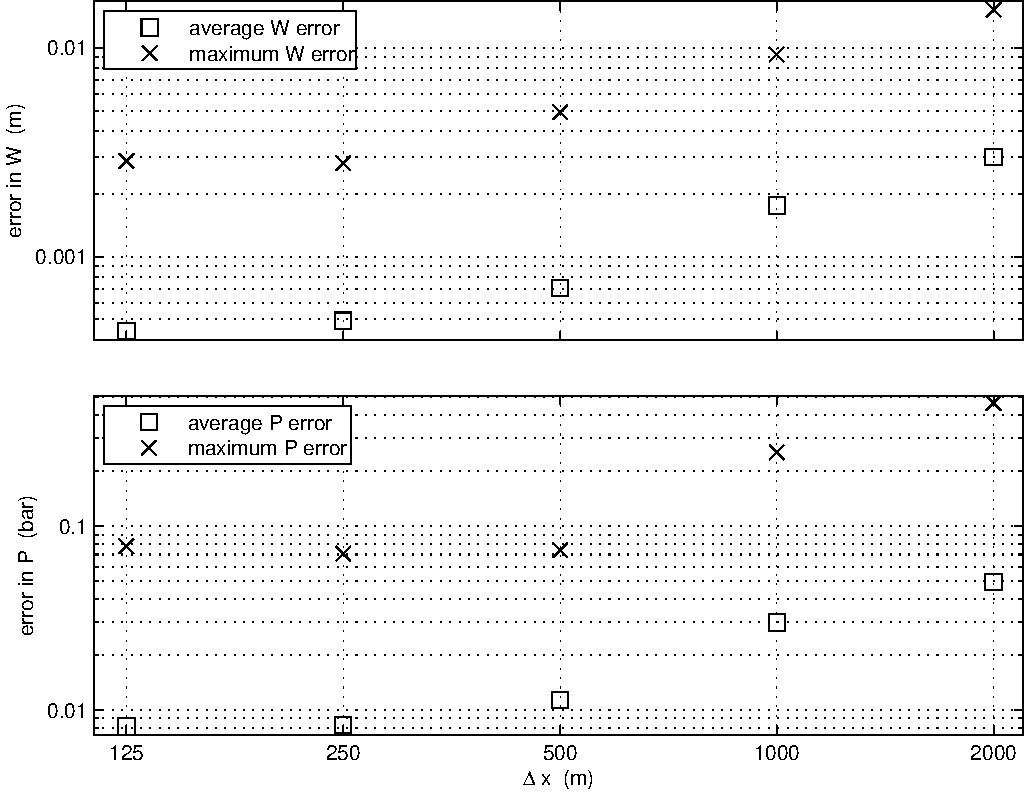
\includegraphics[width=3.0in,keepaspectratio=true]{refineWPpism}
\caption{Average water thickness error $|W-W_{exact}|$ decays as $O(\Delta x^{0.91})$, and average pressure error $|P-P_{exact}|$ decays as $O(\Delta x^{0.92})$, for grids with spacing $250 \le \Delta x = \Delta y \le 2000$ m.}
\label{fig:refineWPpism}
\end{figure}

This convergence evidence suggests that the coupled advection-diffusion-reaction equations for $W$ and $P$ have correctly-implemented numerical schemes.  The rate of convergence is roughly linear (i.e.~about $O(\Delta x^1)$) because largest errors arise at locations of low regularity of the solution, including the radius $r=R_1$ where $P$ abruptly drops from $P_o$, and at the ice sheet margin $r=L$ where there is a jump in the water thickness to zero.

\newcommand{\grnht}{3.8in}

\begin{figure*}[ht]
\mbox{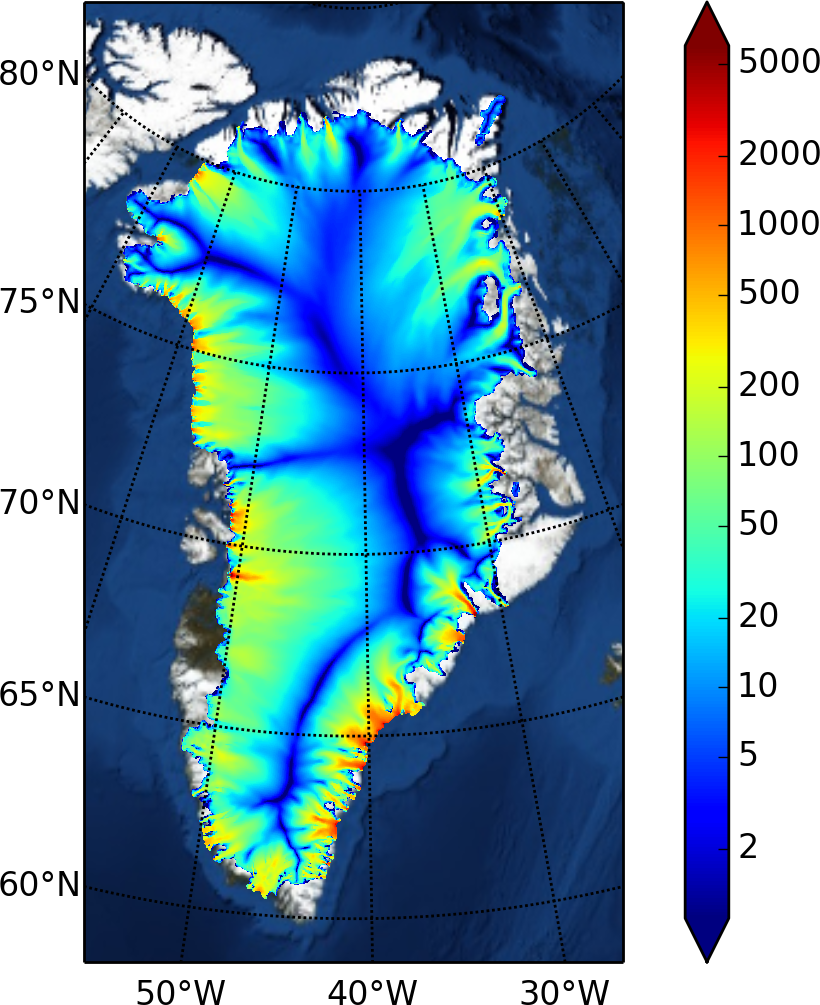
\includegraphics[height=\grnht,keepaspectratio=true]{g2km-init-velsurf-mag} \,
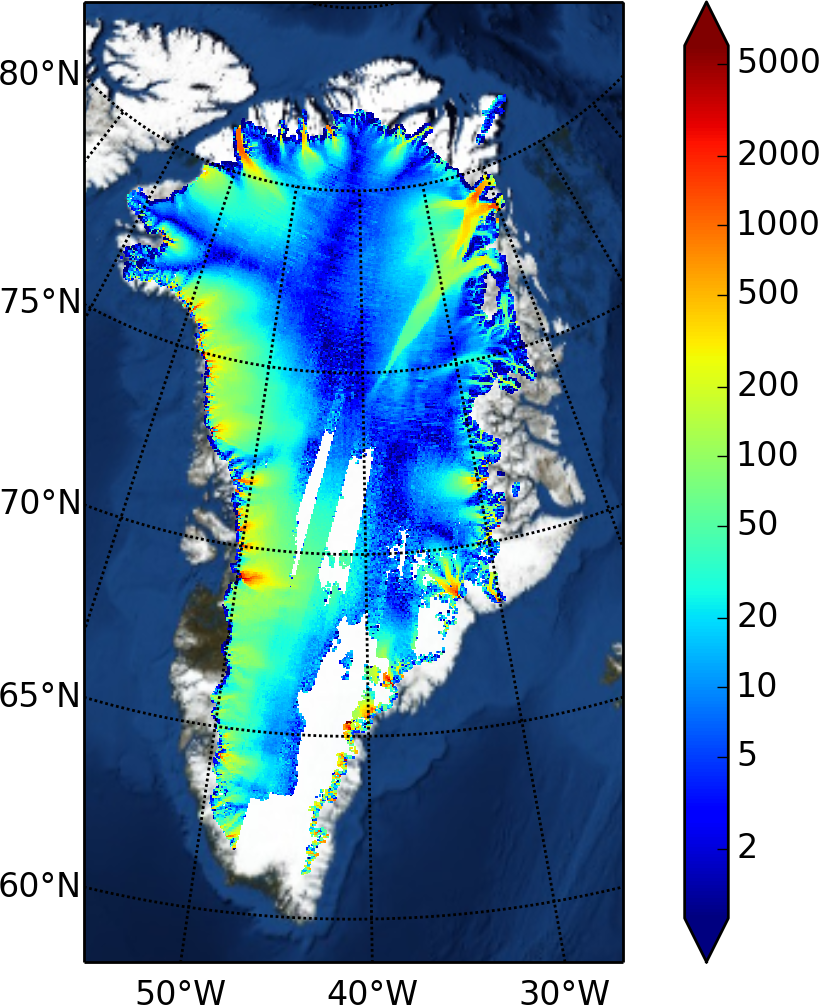
\includegraphics[height=\grnht,keepaspectratio=true]{Greenland-surfvelmag}}
\caption{To evaluate the result of the 2 km grid spun-up ice dynamical model we compare modelled ice speed at the ice surface (left; $\mathrm{m}\,\mathrm{a}^{-1}$) to satellite observations (right; $\mathrm{m}\,\mathrm{a}^{-1}$).}
\label{fig:Greenspinupeval}
\end{figure*}

The rates of convergence for average errors are nearly identical for the higher resolution flux-limited (Koren) scheme and for the first-order upwinding scheme (not shown).  Because our problem is an advection-diffusion problem in which both the advection velocity and the diffusivity are solution-dependent, it is difficult to separate the errors arising from numerical treatments of advection and diffusion.  The first-order upwinding scheme for the advection has much larger numerical diffusivity but this diffusivity is masked by the physical diffusivity.  Based on our verification evidence it is reasonable to choose the simpler first-order upwinding for applications.  It also requires less interprocess communication in our parallel implementation.


\subsection{Application of the model at ice sheet scale}

\subsubsection{Spun-up initial state}  We have applied our mass-conserving hydrology models to the entire present-day Greenland ice sheet at 2 km resolution.  This serves as a nontrivial example showing the implementability of the model at large computational scale with high resolution using real data, and of one-way coupling with ice dynamics.  For simplicity and consistency with prior work, the present-day state of the ice sheet, especially data for the ice thickness, surface mass balance, and surface temperature, were taken from the SeaRISE data set for Greenland (Bindschadler et al., 2013; Nowicki et al., 2013; and references therein).\nocite{Bindschadler2013SeaRISE,Nowicki2013GreenlandSeaRISE}

\begin{figure*}[ht]
\mbox{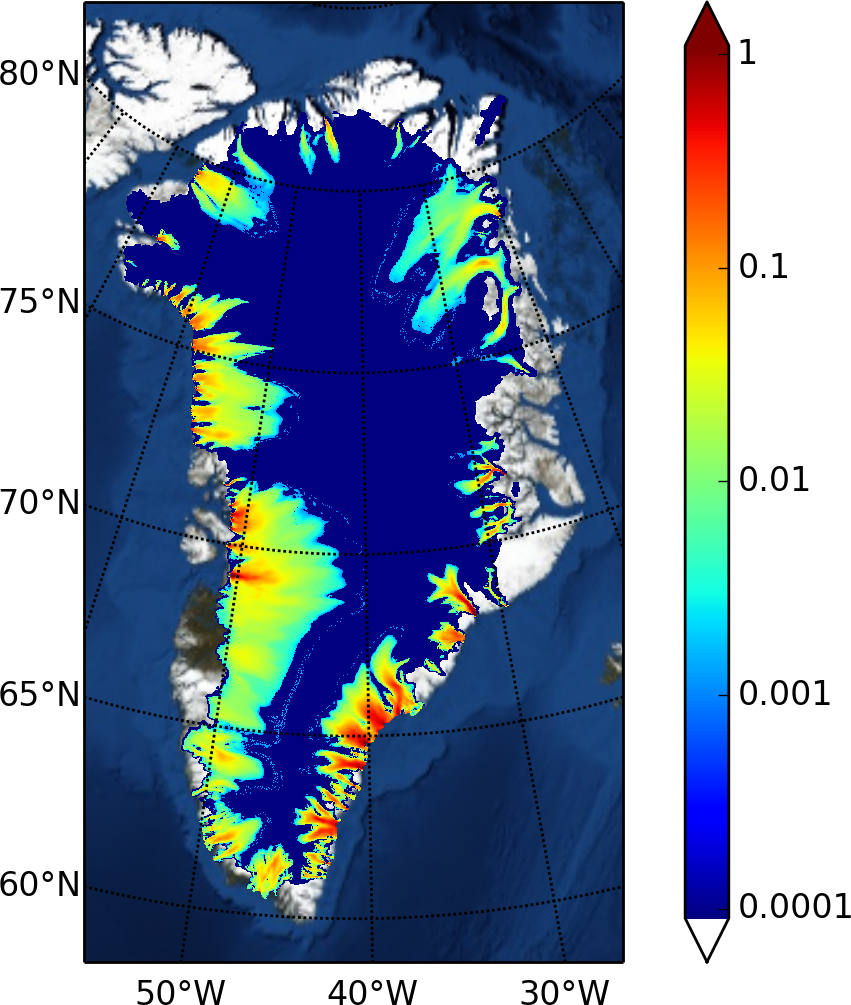
\includegraphics[height=\grnht,keepaspectratio=true]{g2km-init-bmelt} \,
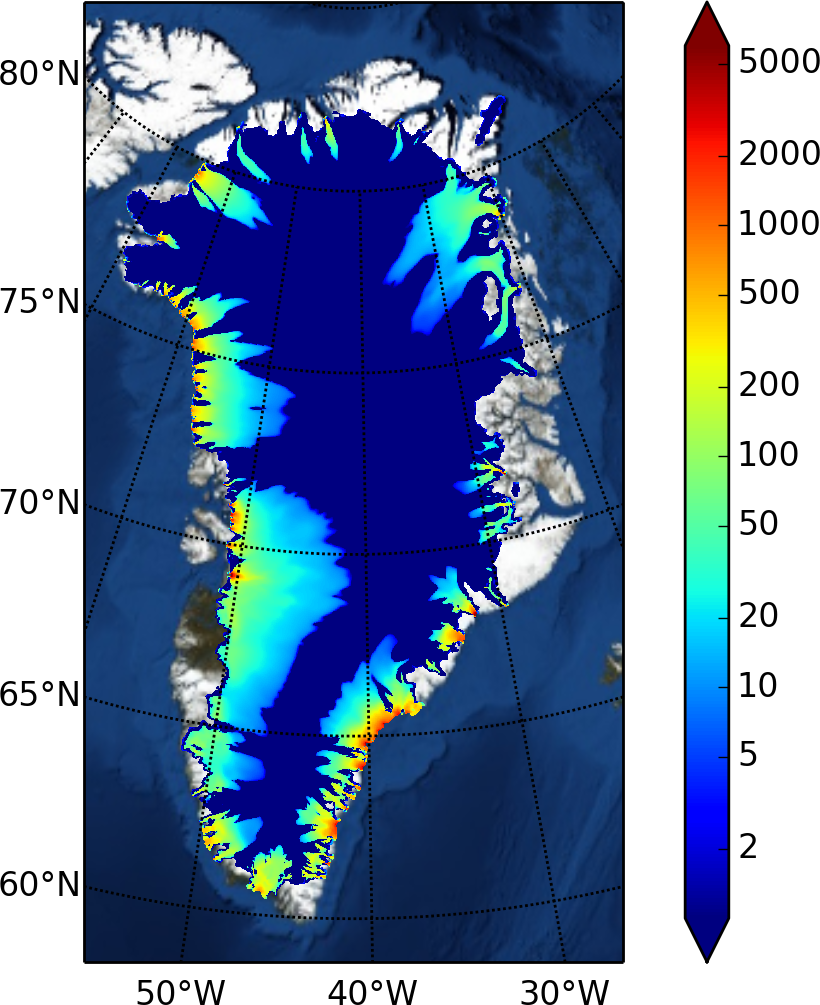
\includegraphics[height=\grnht,keepaspectratio=true]{g2km-init-velbase-mag}}
\caption{The inputs to the hydrology model are the modeled basal melt rate $m/\rho_w$ (left; $\mathrm{m}\,\mathrm{a}^{-1}$) and sliding speed $|\bv_b|$ (right; $\mathrm{m}\,\mathrm{a}^{-1}$) from the spun-up model.}
\label{fig:Greenhydroinputs}
\end{figure*}

The PISM ice dynamics and thermodynamics model \citep{BBssasliding,Winkelmannetal2011,AschwandenBuelerKhroulevBlatter}, using the non-mass-conserving \texttt{null} hydrology model (section \ref{sec:pismdoc}), was applied by grid sequencing to compute a consistent and nearly-steady model of the ice sheet, a ``spun-up'' initial state.  Model choices for ice dynamics, including enhancement factor, sliding law power, and the model for till friction angle, followed those in \cite{AschwandenAdalgeirsdottirKhroulev}.  The present-day climate including surface temperature and mass balance was from \citep{Ettemaetal2009}.  The grid sequence was to run for 50 ka on a 20 km grid, 20 ka on a 10 km grid, 2 ka on a 5 km grid, and finally 200 a on a 2 km grid, with bilinear interpolation of all model fields at each refinement stage.  This whole spinup used 2800 processor-hours on parallel runs of 72 processors on a linux cluster using 2.2 GHz AMD Opteron Processors.  (This represents a small computation for modern clusters which may have more than 100k processors.)

The final 2 km stage, on a horizontal grid of 1.05 million grid points, used uniform 10 m vertical spacing so that the ice sheet flow was modelled on a structured 3D grid of 460 million grid points (e.g.~locations where ice temperature and velocity were computed).  In the last 100 a of the final stage the ice sheet volume varied by less than $0.04$ percent.  Other more active measures showed stability during the last 100 a at the level of less than one percent (e.g.~the area of temperate base and the maximum ice velocity over the whole sheet) to at most a few percent (the floating ice area).
 
The results of this whole-ice-sheet spinup were validated by comparing results to present-day observations.  Though the model is in nearly steady state, the actual ice sheet may not be as close to steady.  The spun-up ice sheet volume of $3.094\times 10^{6}\,\textrm{km}^3$ is close to the present-day volume of $3.088\times 10^{6}\,\textrm{km}^3$ computed from the SeaRISE data on the same grid.  However, in describing more careful validation measures for similar 2 km PISM model runs, \cite{AschwandenAdalgeirsdottirKhroulev} observe that volume alone is inadequate for model validation.  A better evaluation of dynamical quality is shown in Figure \ref{fig:Greenspinupeval}, which compares the modeled and observed surface speed.  We see that, the extent of the Northeast Greenland ice stream is smaller than observed, and the distribution of flow in Western Greenland outlet glaciers differs from the observed pattern.  Our model uses no spatially-variable parameter values such as basal shear stresses found by inversion of surface velocities.

\begin{figure*}[ht]
\mbox{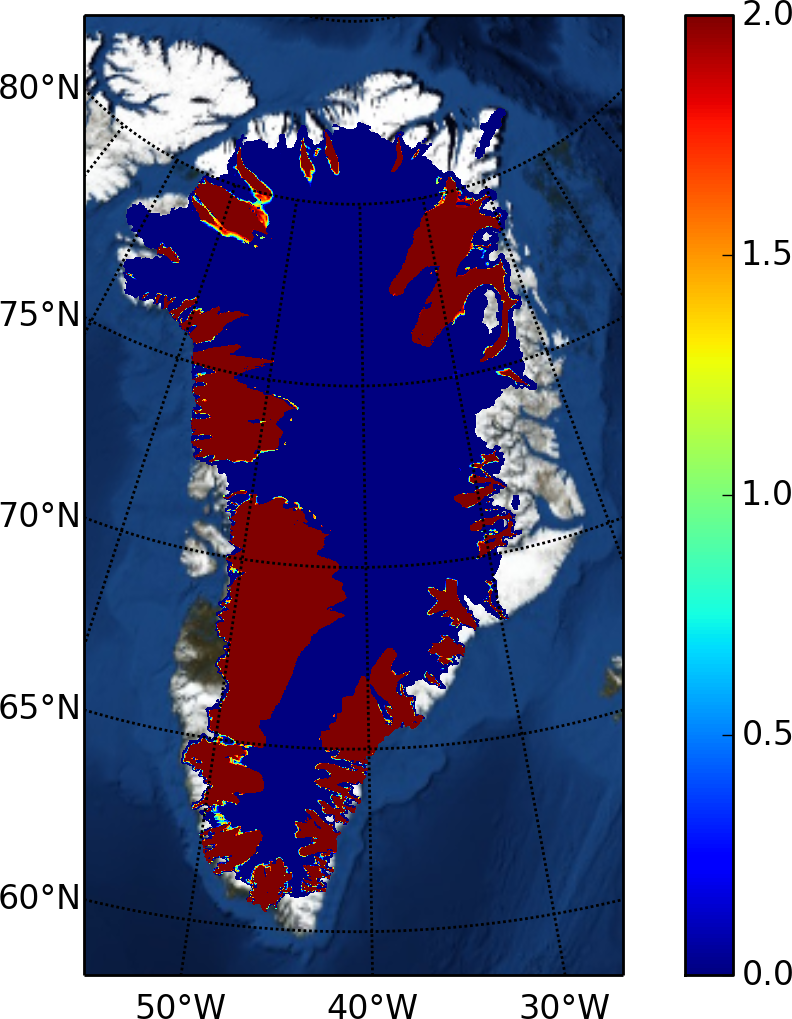
\includegraphics[height=\grnht,keepaspectratio=true]{routing-decoupled-tillwat} \,
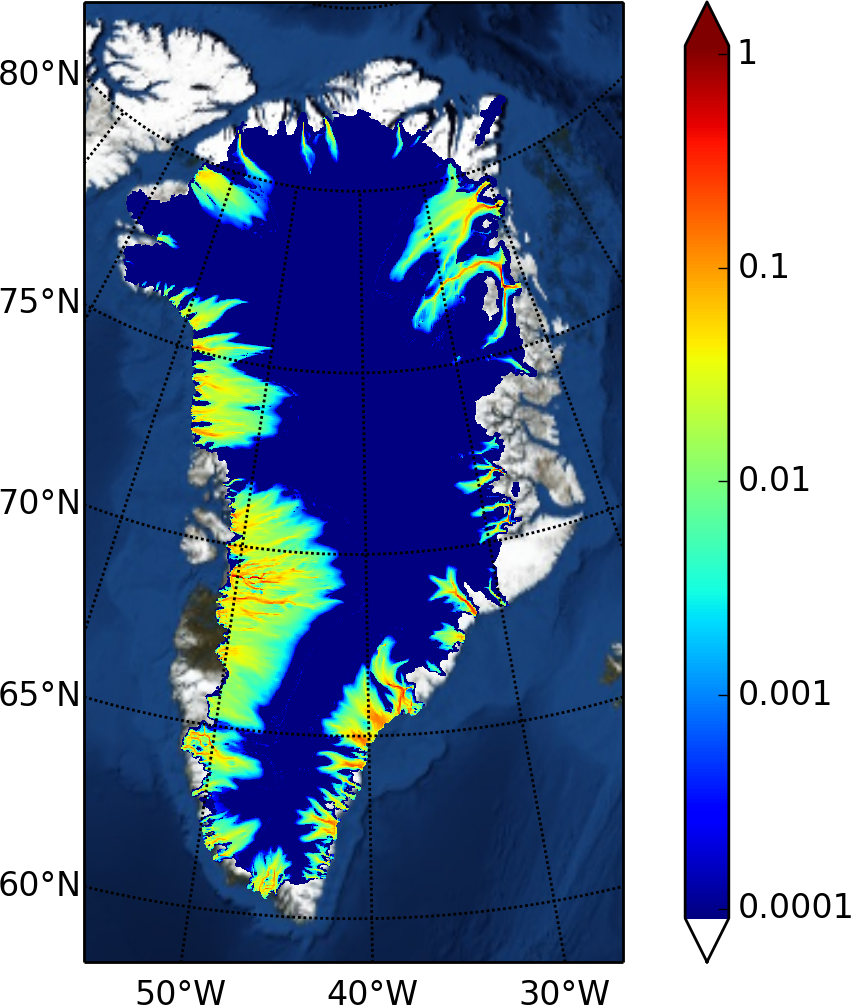
\includegraphics[height=\grnht,keepaspectratio=true]{routing-decoupled-bwat}}
\caption{Outputs from the \texttt{routing} hydrology model are the modelled till-stored water layer thickness $\Wtil$ (left; $\mathrm{m}$) and modelled transportable water layer thickness $W$ (right; $\mathrm{m}$).}
\label{fig:Greenroutingresults}
\end{figure*}

The spun-up initial state includes, in particular, modelled ice thickness $H$, basal melt rate $m$, and sliding velocity $|\bv_b|$; the latter two fields are shown in Figure \ref{fig:Greenhydroinputs}.  We note that the areas of sliding roughly coincide with areas of basal melt because modeled basal resistance comes from the yield stress parameterized in section \ref{sec:tillmechanics}.

\subsubsection{Experimental setup}  We then used the fields $H$, $m$, $|\bv_b|$ as steady data in five model-year runs of our mass-conserving hydrology \texttt{routing} and \texttt{distributed} models.  Because these fields were fixed, only one-way coupling is tested here.  That is, a steady ice dynamics model fed its fields to an evolving subglacial hydrology model.  The hydrology model was initialized with the $\Wtil$ values from the spun-up state, but with $W=0$ initial values (for both models) and $P=0$ initial values (for \texttt{distributed}).

These runs had 1.05 million subglacial hydrology grid points at which variables $W$, $\Wtil$, and $P$ were recomputed at each time-step according to the numerical model described in section \ref{sec:num}.  In both \texttt{routing} and \texttt{distributed} models the modelled hydrological system became quite steady after the first three model years.  The adaptively-determined time-steps for the hydrology model reached a steady level of 4 model hours for the \texttt{routing} model based on maximum subglacial water speeds $|\bV|$ of 0.05 $\text{m}\,\text{s}^{-1}$ and maximum diffusivity $D$ of 10.6 $\text{m}^2\,\text{s}^{-1}$.  For the complete \texttt{distributed} model the time steps were actually slightly longer than \texttt{routing} primarily because the routing model concentrates large water amounts, and thus fluxes, along steepest-descent paths.  In the \texttt{distributed} model the time steps were about 6 model hours based on speeds $|\bV|$ of 0.03 $\text{m}\,\text{s}^{-1}$ and substantially-smaller maximum diffusivities of about $D$ of 0.25 $\text{m}^2\,\text{s}^{-1}$.  (Note comments on the actual diffusivity of advective fluxes in section \ref{sec:steady}.  Also, higher water velocities $\bV$ were seen in the \Nbreen case in section \ref{sec:num}, based on additional simulated surface water input added to the thermodynamically-generated basal melt rate \citep{vanPeltthesis}.  In that tidewater glacier case the pressure-evolution time-steps are seen to be substantially shorter than the mass-conservation time steps.)

\subsubsection{\texttt{routing} results}  The final values of $\Wtil$ and $W$ for the \texttt{routing} run are shown in Figure \ref{fig:Greenroutingresults}.  We see that the till is fully saturated ($\Wtil=2$ m) in essentially all areas where basal melt occurs.  In the outlet glacier areas the transportable water $W$ concentrates along curves of steepest descent of the hydraulic potential; this effect is seen in detail in Figure \ref{fig:Greenroutingdetail}.  The grid resolution of 2 km, while very high for contemporary ice dynamics models, still represents a significant spatial ``smearing'' of the flow pathways.  Specifically, though relatively few areas have $W>1$, the continuum limit of the model would be expected to have $W\gg 1$ in concentrated pathways of a few meters to tens of meters width.  These effects are seen in detail in Figure \ref{fig:Greenroutingdetail}.

\begin{figure*}[ht]
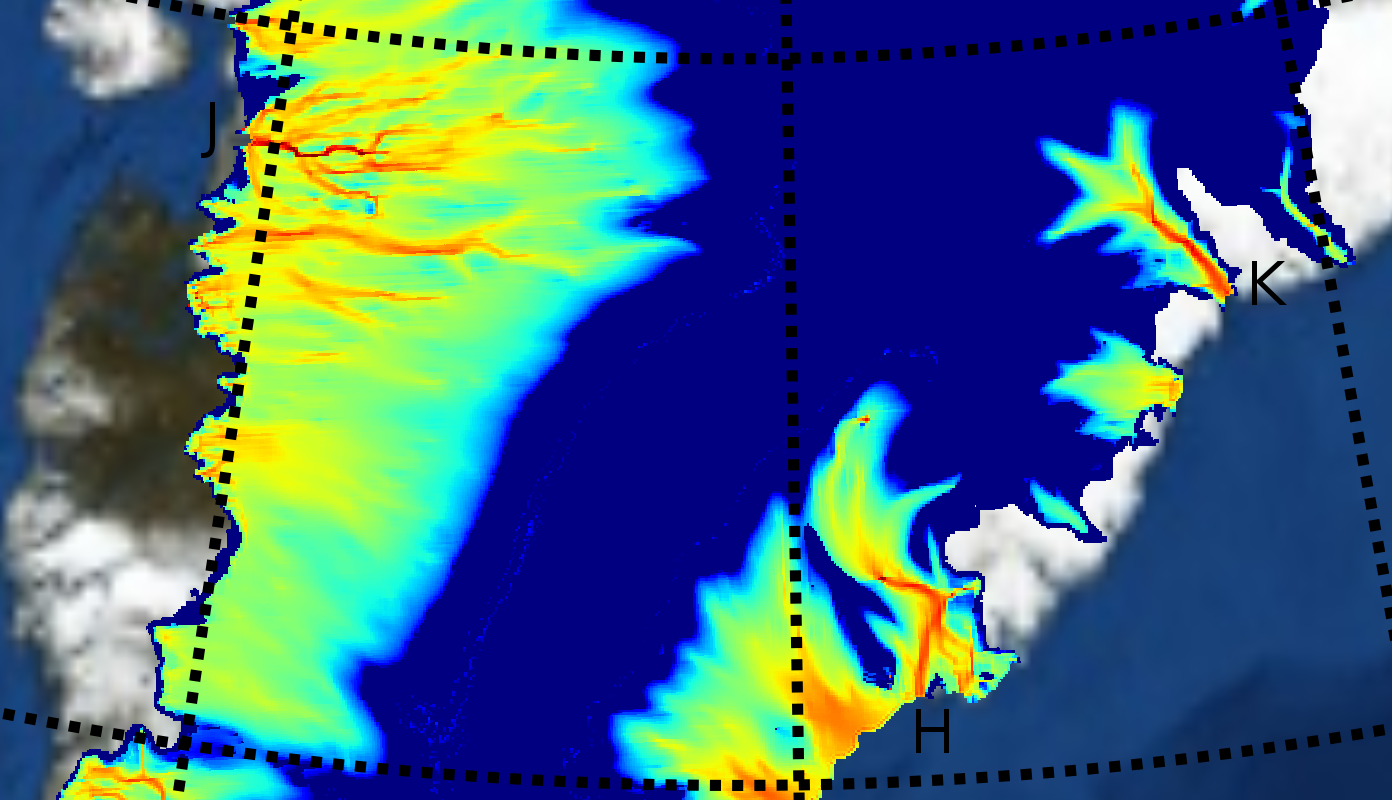
\includegraphics[height=2.7in,keepaspectratio=true]{detail-routing-decoupled-bwat}
\caption{Detail of transportable water $W$ plotted in Figure \ref{fig:Greenroutingresults}, covering Jakobshavn (J), Helheim (H), and Kangerdlugssuaq (K) outlet glaciers}
\label{fig:Greenroutingdetail}
\end{figure*}

On the one hand this model could be regarded as a minimal ``conduit-like'' description of the subglacial flow, because of these model concentrated pathways.  On the other hand, as noted in the introduction, there is no ``R-channel'' mechanism used in this paper; in that mechanism the dissipation heating of the flowing water would generate wall melt-back to hold the channel open.  Thus the time-dependence and flux magnitudes in the model are not ``R-channel''-like.  At a more basic level, the authenticity of subglacial ``channel'' geometry here is determined primarily by the bedrock elevation detail provided by the SeaRISE data set, which is limited; this effect is severe in the Eastern outlet glaciers (Helheim and Kangerdlugssuaq) shown in Figure \ref{fig:Greenroutingdetail}.

\subsubsection{\texttt{distributed} results}  The final values of $W$ and the relative water pressure $P/P_o$ for the five model-year \texttt{distributed} run are shown in Figure \ref{fig:Greendistributedresults}.  Again the till is full ($\Wtil=\Wtilmax=2$ m) in essentially all areas where basal melt occurs, so $\Wtil$ is not shown because it is identical to that in the \texttt{routing} model in this one-way coupled case.  (Note the simple $\Wtil$ evolution equation given in section \ref{sec:capacity}.)

Recall that $|\bv_b|$ determines the pressure drop caused by cavitation.  The tendency of this effect to spread out the water $W$, relative to the \texttt{routing} model, is clearly seen in the \texttt{distributed} results in Figure \ref{fig:Greendistributedresults}.  There is no strong concentration of $W$ along curves of steepest descent of the hydraulic potential.  This result is strongly dependent on the opening and closing parameters in the \texttt{distributed} model, especially parameters $c_1,c_2,\phi_0,W_r$; see Tables \ref{tab:constants} and \ref{tab:correspondence}.  (These are in addition to the Darcy flux model parameters $\alpha,\beta,k$ already used in the \texttt{routing} model.)  Parameter identification through observed data is obviously needed, but it is beyond the scope of the current paper.

\begin{figure*}[ht]
\mbox{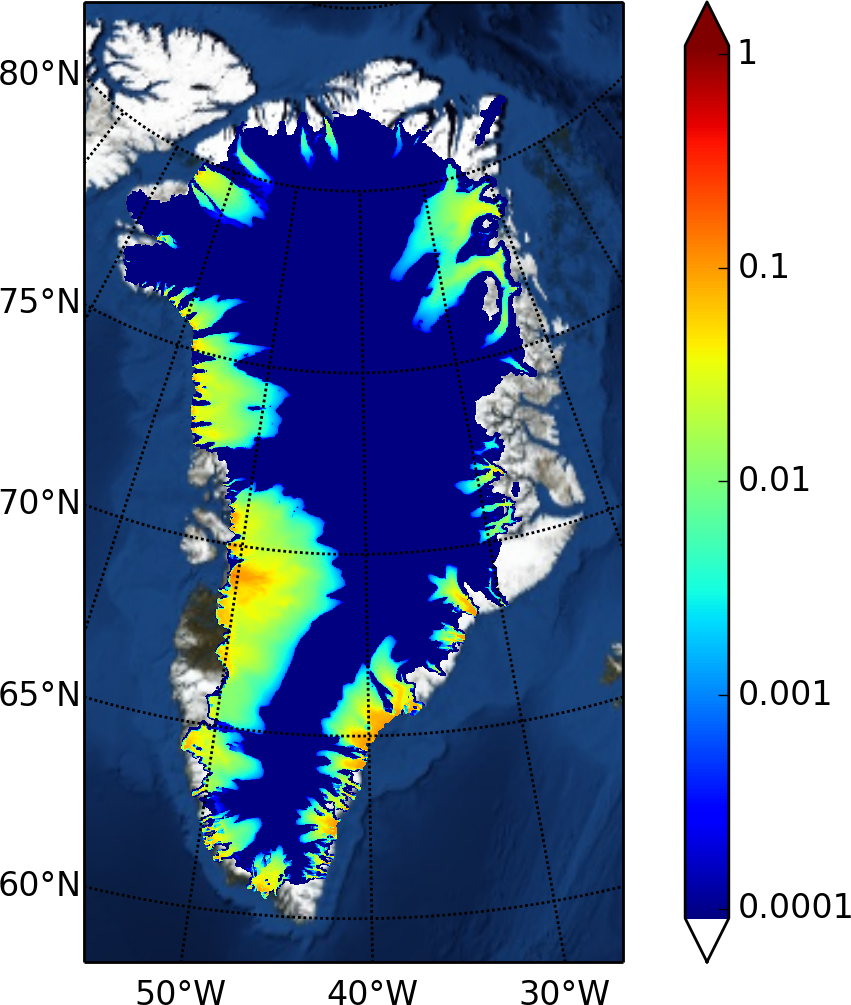
\includegraphics[height=\grnht,keepaspectratio=true]{distributed-decoupled-bwat} \,
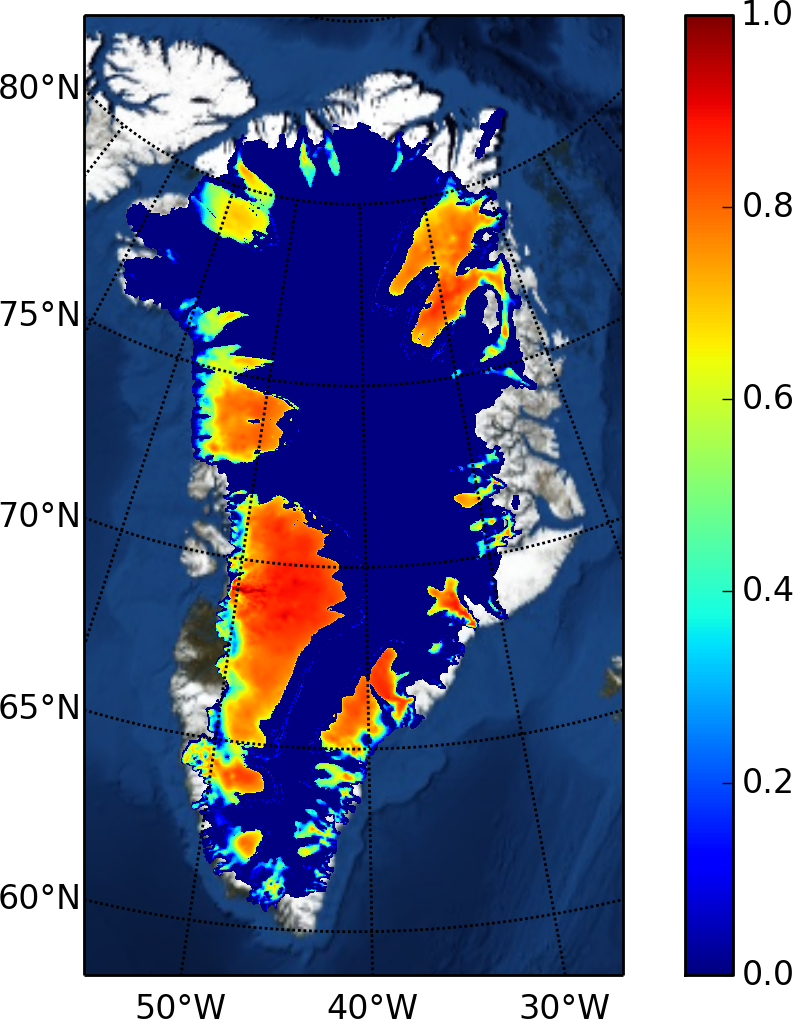
\includegraphics[height=\grnht,keepaspectratio=true]{distributed-decoupled-bwprel}}
\caption{Outputs from the \texttt{distributed} hydrology model are the modelled till-stored water layer thickness $\Wtil$ (not shown because it is identical to the result from the \texttt{routing} model in this case; see text), the modelled transportable water layer thickness $W$ (left; $\mathrm{m}$), and the modelled transportable water layer pressure relative to overburden pressure $P/P_o$ (right).}
\label{fig:Greendistributedresults}
% note routing-decoupled-bwat.png is not shown but it really is identical to routing-decoupled-tillwat.png
\end{figure*}

As a final observation about the \texttt{distributed} model results, we examine the local relationship between water amount $W$ and pressure $P$.  Though the model is near steady state, the basal melt rate, sliding speed, and overburden pressure all show the large spatial variations which are characteristic of a real ice sheet.

\newcommand{\myheight}{2.0in}
\begin{figure*}[ht]
\mbox{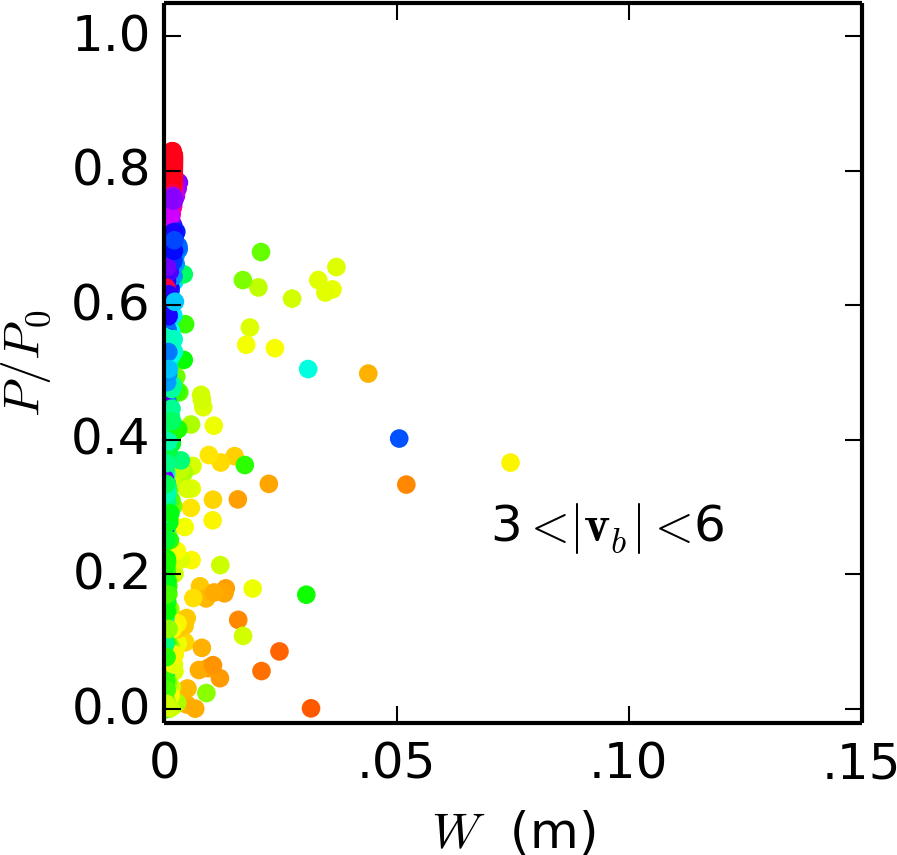
\includegraphics[height=\myheight,keepaspectratio=true]{bin1-g2km} \, 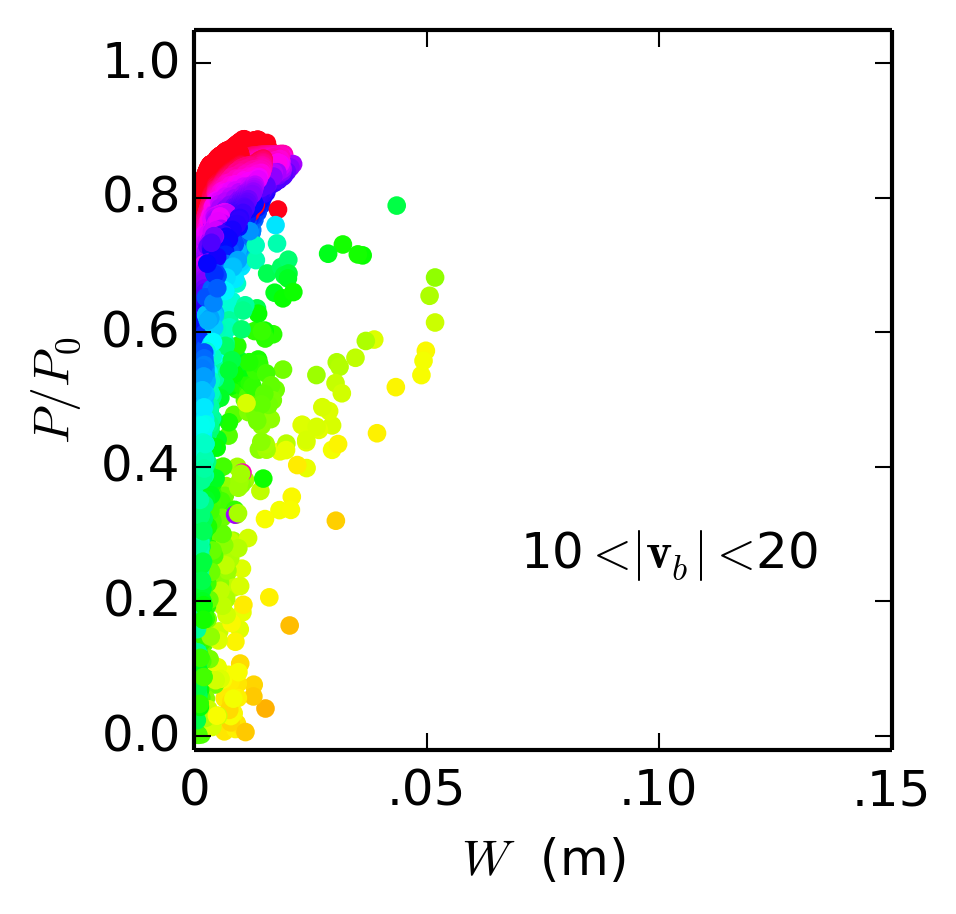
\includegraphics[height=\myheight,keepaspectratio=true]{bin10-g2km} \, 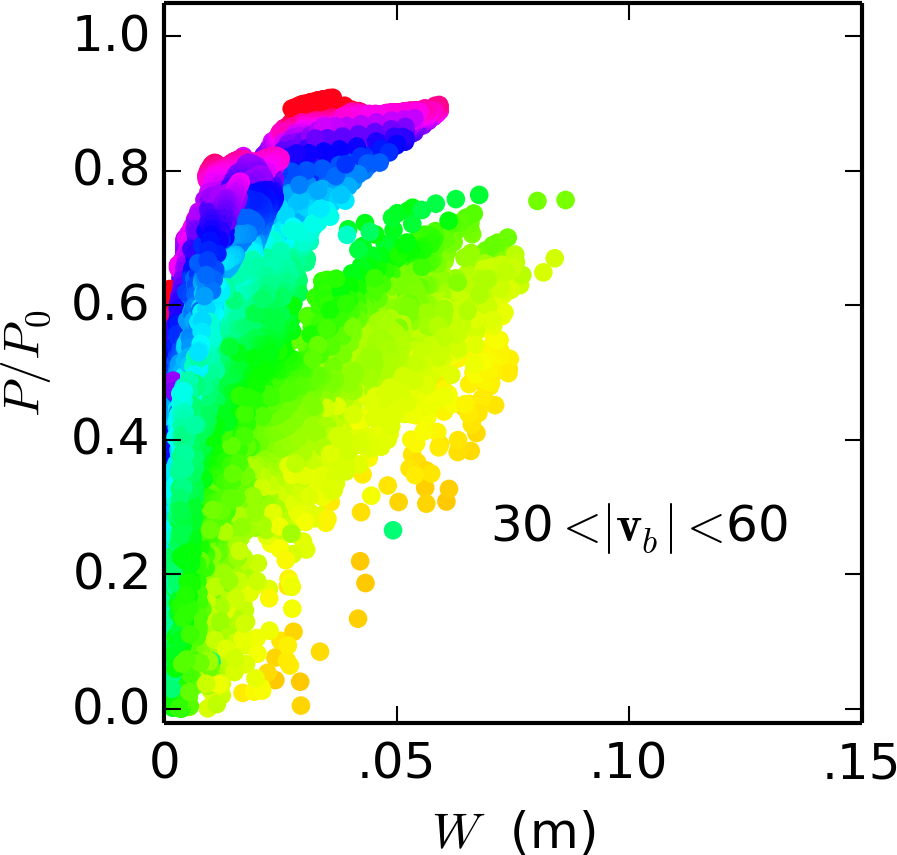
\includegraphics[height=\myheight,keepaspectratio=true]{bin30-g2km}}
\mbox{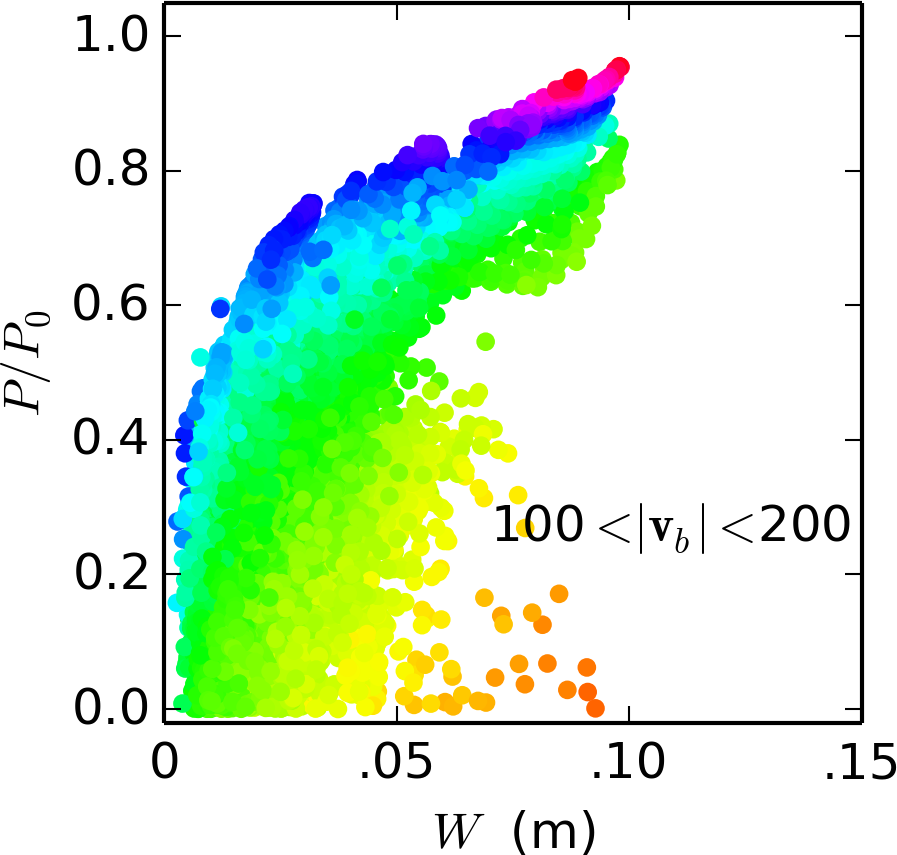
\includegraphics[height=\myheight,keepaspectratio=true]{bin100-g2km} \,
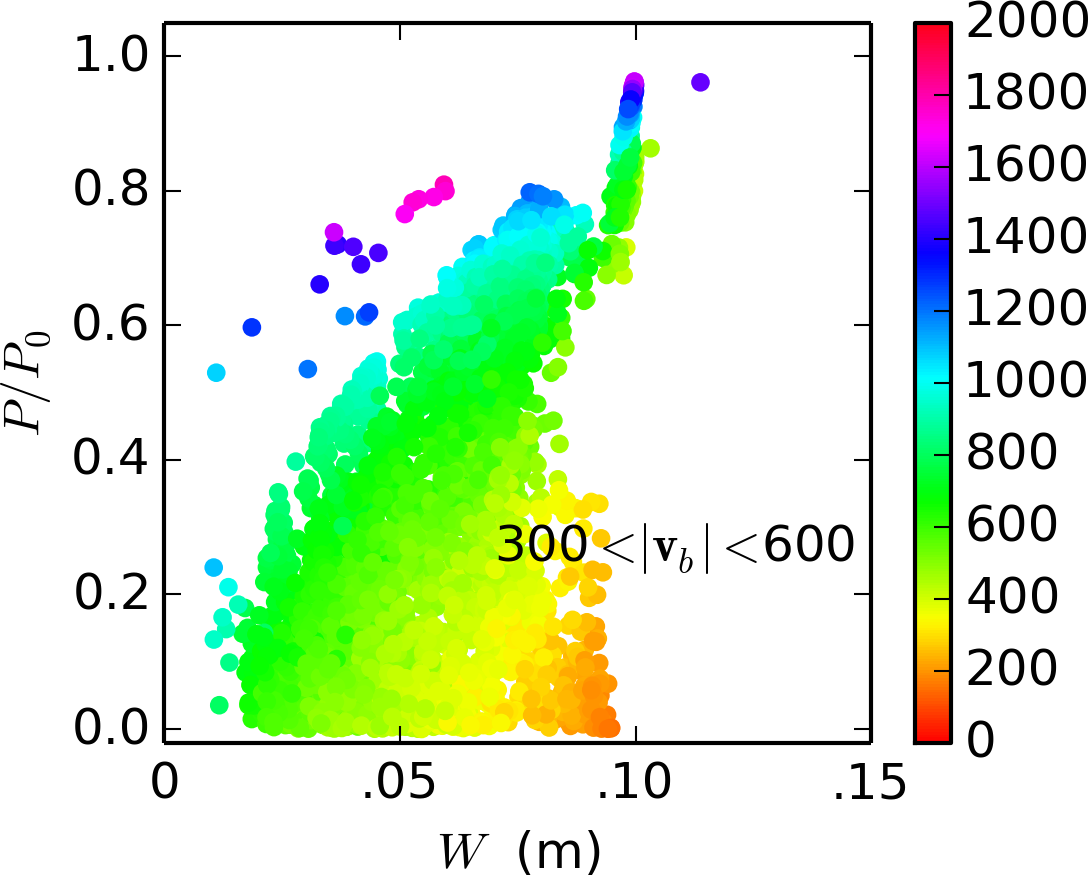
\includegraphics[height=2.05in,keepaspectratio=true]{bin300-g2km}}
\caption{Scatter plots of $(W,P)$ pairs for all cells at end of a 5 model year steady-input simulation on a 2 km grid for the whole Greenland ice sheet using roughness scale $W_r = 0.1$ m.  Each scatter plot shows the pairs for a select range of ice sliding speeds, as indicated.  Points are colored by ice thickness using a common scale shown beside last figure.}
\label{fig:GreenisPofW}
\end{figure*}

Figure \ref{fig:GreenisPofW} shows that if we ``bin'' pairs $(W,P)$ by relatively-narrow sliding velocity ranges, as shown in each scatter plot, then there is usually a rough increasing relationship between $W$ and the relative pressure $P/P_o$.  Recall that in exact steady state the equation \eqref{eq:PofWsteady} applies; see also Figures \ref{fig:psteady-vb} and \ref{fig:psteady-Po}.  At fast-sliding locations the water amount is often comparable to the bed roughness scale $W_r$.  For low sliding velocities we see generally lower water amounts ($W \lesssim W_r/10$) but a full range of pressures.  Furthermore we can observe that in thick ice with high overburden pressure the pressure $P$ is close to overburden even if there is fast sliding.  Locations with high sliding, high water amount, and low pressure also have low ice thickness.  Figure \ref{fig:GreenisPofW} would show even more scatter if the run were not close to steady state, such as if there were time-varying surface melt input into the subglacier \citep{vanPeltthesis}.

It would be possible to implement a model without a pressure evolution equation like \eqref{eq:regpressureequation}, and instead use \eqref{eq:PofWsteady} as a prescribed relation $P(W)$.  However, we prefer such a local relationship to ``emerge'' in steady state, as here.  Tests of the model with time-dependent inputs clearly suggest the importance of a full pressure evolution equation to modeling response to a seasonal surface melt cycle \citep{vanPeltthesis}.


\conclusions  \label{sec:conclusion}  The literature of subglacial hydrology modeling has grown rapidly in the last five years.  In this context the current paper, which documents additions made to the Parallel Ice Sheet Model in its 0.6 version released February 2014, is both novel and comprehensive, despite primarily describing the details of a PISM submodel.  It is novel in these features:\begin{itemize}
\item parallel implementation in two horizontal dimensions at scale (sections \ref{sec:num} and \ref{sec:results}) of a coupled till-and-linked-cavities model,
\item a new analysis of steady state explaining the degree to which a functional relationship $P(W)$ is justified (section \ref{sec:steady}),
\item an exact solution of the coupled mass and pressure equations of the distributed model in the steady angularly-symmetric case (section \ref{sec:steady}), plus verification using this solution (section \ref{sec:results}), and
\item an englacial porosity regularization which is shown to allow a practical numerical model in which physically-motivated bounds $0\le P \le P_o$ hold at all times (sections \ref{sec:capacity}, \ref{sec:closures}, and \ref{sec:num}).
\end{itemize}
We believe, however, that the comprehensive treatment here of certain subjects is also important.  We assert that
\begin{itemize}
\item we have clarified the relationship of several ``closures'' which turn morphological ideas about the subglacial aquifer into concrete pressure equations (section \ref{sec:closures}), and
\item we have implemented a common extension of several seemly-disparate published models (section \ref{sec:newmodel}).
\end{itemize}
On the other hand, a deliberate limitation in scope of the current paper is that we demonstrate only one-way coupling: the PISM ice flow and thermodynamics model feeds basal melt rate and sliding speed values to the hydrology model.  Two-way coupling in a high-resolution model for the whole of the Greenland ice sheet will appear in future work.

\begin{acknowledgements}
The first author was supported by NASA grant \#NNX13AM16G.  This work was supported by a grant of high-performance computing resources from the Arctic Region Supercomputing Center.  Constantine Khroulev helped with the PISM implementation.  Discussions with, and detailed comments by, Andy Aschwanden, Tim Bartholomaus, and Martin Truffer were much appreciated.
\end{acknowledgements}


%\bibliography{ice-bib}  % generally requires link to pism/doc/ice-bib.bib
%\bibliographystyle{copernicus}

\begin{thebibliography}{68}
\providecommand{\natexlab}[1]{#1}
\providecommand{\url}[1]{{\tt #1}}
\providecommand{\urlprefix}{URL }
\expandafter\ifx\csname urlstyle\endcsname\relax
  \providecommand{\doi}[1]{doi:\discretionary{}{}{}#1}\else
  \providecommand{\doi}{doi:\discretionary{}{}{}\begingroup
  \urlstyle{rm}\Url}\fi

\bibitem[{Ascher and Petzold(1998)}]{AscherPetzold}
Ascher, U. and Petzold, L.: Computer {M}ethods for {O}rdinary {D}ifferential
  {E}quations and {D}ifferential-algebraic {E}quations, SIAM Press,
  Philadelphia, PA, 1998.

\bibitem[{Aschwanden et~al.(2012)Aschwanden, Bueler, Khroulev, and
  Blatter}]{AschwandenBuelerKhroulevBlatter}
Aschwanden, A., Bueler, E., Khroulev, C., and Blatter, H.: An enthalpy
  formulation for glaciers and ice sheets, J. Glaciol., 58, 441--457,
  \doi{10.3189/2012JoG11J088}, 2012.

\bibitem[{Aschwanden et~al.(2013)Aschwanden, Adalgeirsd{\'o}ttir, and
  Khroulev}]{AschwandenAdalgeirsdottirKhroulev}
Aschwanden, A., Adalgeirsd{\'o}ttir, G., and Khroulev, C.: Hindcasting to
  measure ice sheet model sensitivity to initial states, The Cryosphere, 7,
  1083--1093, \doi{10.5194/tc-7-1083-2013}, 2013.

\bibitem[{Balay et~al.(2011)}]{petsc-user-ref}
Balay, S. et~al.: {PETS}c {U}sers {M}anual, Tech. Rep. ANL-95/11 - Revision
  3.2, Argonne National Laboratory, 2011.

\bibitem[{Bartholomaus et~al.(2008)Bartholomaus, Anderson, and
  Anderson}]{Bartholomausetal2008}
Bartholomaus, T.~C., Anderson, R.~S., and Anderson, S.~P.: Response of glacier
  basal motion to transient water storage, Nature Geosci., 1, 33--37,
  \doi{10.1038/ngeo.2007.52}, 2008.

\bibitem[{Bartholomaus et~al.(2011)Bartholomaus, Anderson, and
  Anderson}]{Bartholomausetal2011}
Bartholomaus, T.~C., Anderson, R.~S., and Anderson, S.~P.: Growth and collapse
  of the distributed subglacial hydrologic system of {K}ennicott {G}lacier,
  {A}laska, {USA}, and its effects on basal motion, J. Glaciol., 57, 985--1002,
  2011.

\bibitem[{Bindschadler and twenty-seven others(2013)Bindschadler
  et~al.}]{Bindschadler2013SeaRISE}
Bindschadler, R. et~al.: Ice-sheet model sensitivities to environmental forcing
  and their use in projecting future sea-level ({T}he {S}ea{RISE} {P}roject),
  J. Glaciol, 59, 195--224, 2013.

\bibitem[{Bueler(2014)}]{Bueler2014correspondence}
Bueler, E.: Correspondence: Extensions of the lumped subglacial-englacial
  hydrology model of {B}artholomaus, et al.~(2011), submitted to J.~Glaciol.,
  2014.

\bibitem[{Bueler and Brown(2009)}]{BBssasliding}
Bueler, E. and Brown, J.: Shallow shelf approximation as a ``sliding law'' in a
  thermodynamically coupled ice sheet model, J. Geophys. Res., 114, f03008,
  doi:10.1029/2008JF001179, 2009.

\bibitem[{Bueler et~al.(2005)}]{BLKCB}
Bueler, E. et~al.: Exact solutions and numerical verification for isothermal ice sheets,
  J. Glaciol., 51, 291--306, 2005.

\bibitem[{Clarke(2003)}]{Clarke2003}
Clarke, G.~K.: Hydraulics of subglacial outburst floods: new insights from the
  {Spring-Hutter} formulation, J. Glaciol., 49, 299--313,
  \doi{10.3189/172756503781830728}, 2003.

\bibitem[{Clarke(2005)}]{Clarke05}
Clarke, G.: Subglacial processes, Annu. Rev. Earth Planet. Sci., 33,
  247--276, \doi{10.1146/annurev.earth.33.092203.122621}, 2005.

\bibitem[{Creyts and Schoof(2009)}]{CreytsSchoof2009}
Creyts, T. and Schoof, C.: Drainage through subglacial water sheets, J.
  Geophys. Res., 114, \doi{10.1029/2008JF001215}, 2009.

\bibitem[{Cuffey and Paterson(2010)}]{CuffeyPaterson}
Cuffey, K.~M. and Paterson, W. S.~B.: The {P}hysics of {G}laciers, Elsevier,
  4th edn., 2010.

\bibitem[{Das et~al.(2008)Das, Joughin, Behn, Howat, King, Lizarralde, and
  Bhatia}]{Dasetal08}
Das, S.~B., Joughin, I., Behn, M.~D., Howat, I.~M., King, M.~A., Lizarralde,
  D., and Bhatia, M.~P.: {Fracture Propagation to the Base of the Greenland Ice
  Sheet During Supraglacial Lake Drainage}, Science, 320, 778--781,
  \doi{10.1126/science.1153360}, 2008.

\bibitem[{de~Fleurian et~al.(2014)de~Fleurian, Gagliardini, Zwinger, Durand,
  Le~Meur, Mair, and R{\aa}back}]{deFleurianetal2014}
de~Fleurian, B., Gagliardini, O., Zwinger, T., Durand, G., Le~Meur, E., Mair,
  D., and R{\aa}back, P.: A double continuum hydrological model for glacier
  applications, The Cryosphere, 8, 137--153, \doi{10.5194/tc-8-137-2014}, 2014.

\bibitem[{Ettema et~al.(2009)}]{Ettemaetal2009}
Ettema J. et~al.: Higher surface mass balance of the Greenland ice sheet
  revealed by high-resolution climate modeling, Geophys. Res. Lett., 36, L12501,
  \doi{10.1029/2009GL038110}, 2009.

\bibitem[{Evans(1998)}]{Evans}
Evans, L.~C.: Partial {D}ifferential {E}quations, Graduate Studies in
  Mathematics, American Mathematical Society, 1998.

\bibitem[{Flowers and Clarke(2002{\natexlab{a}})}]{FlowersClarke2002_theory}
Flowers, G.~E. and Clarke, G. K.~C.: A multicomponent coupled model of glacier
  hydrology 1. {T}heory and synthetic examples, J. Geophys. Res., 107, 2287,
  \doi{10.1029/2001JB001122}, 2002{\natexlab{a}}.

\bibitem[{Flowers and Clarke(2002{\natexlab{b}})}]{FlowersClarke2002_trapridge}
Flowers, G.~E. and Clarke, G. K.~C.: A multicomponent coupled model of glacier
  hydrology 2. {A}pplication to {T}rapridge {G}lacier, {Y}ukon, {C}anada, J.
  Geophys. Res., 107, 2288, \doi{10.1029/2001JB001124}, 2002{\natexlab{b}}.

\bibitem[{Fountain et~al.(2005)}]{Fountainetal2005}
Fountain, A., et al.: Fractures as the main pathways of water flow in temperate glaciers, Nature 433, 618--621, \doi{doi:10.1038/nature03296}, 2005.

\bibitem[{Goeller et~al.(2013)Goeller, Thoma, Grosfeld, and
  Miller}]{Goelleretal2013}
Goeller, S., Thoma, M., Grosfeld, K., and Miller, H.: A balanced water layer
  concept for subglacial hydrology in large-scale ice sheet models, The
  Cryosphere, 7, 1095--1106, 2013.

\bibitem[{Greve and Blatter(2009)}]{GreveBlatter2009}
Greve, R. and Blatter, H.: Dynamics of {I}ce {S}heets and {G}laciers, Advances
  in Geophysical and Environmental Mechanics and Mathematics, Springer, 2009.

\bibitem[{Harper et~al.(2010)Harper, Bradford, Humphrey, and
  Meierbachtol}]{Harperetal2010}
Harper, J., Bradford, J., Humphrey, N., and Meierbachtol, T.: Vertical
  extension of the subglacial drainage system into basal crevasses, Nature,
  467, 579--582, \doi{10.1038/nature09398}, 2010.

\bibitem[{Hewitt(2011)}]{Hewitt2011}
Hewitt, I.~J.: Modelling distributed and channelized subglacial drainage: the
  spacing of channels, J. Glaciol., 57, 302--314, 2011.

\bibitem[{Hewitt(2013)}]{Hewitt2013}
Hewitt, I.~J.: Seasonal changes in ice sheet motion due to melt water
  lubrication, Earth Planet. Sci. Lett., 371--372, 16--25,
  \doi{10.1016/j.epsl.2013.04.022}, 2013.

\bibitem[{Hewitt et~al.(2012)Hewitt, Schoof, and Werder}]{Hewittetal2012}
Hewitt, I.~J., Schoof, C., and Werder, M.~A.: Flotation and free surface flow
  in a model for subglacial drainage. {P}art {II}: {C}hannel flow, J. Fluid
  Mech., 702, 157--188, 2012.

\bibitem[{Hooke et~al.(1997)}]{Hookeetal1997}
Hooke, R. et~al.: Rheology of
  till beneath {S}t\"orglaciaren, {S}weden, J. Glaciol., 43, 172--179, 1997.

\bibitem[{Hundsdorfer and Verwer(2010)}]{HundsdorferVerwer2010}
Hundsdorfer, W. and Verwer, J.~G.: Numerical {S}olution of {T}ime-{D}ependent
  {A}dvection-{D}iffusion-{R}eaction {E}quations, Springer Series in
  Computational Mathematics, Springer, 2010.

\bibitem[{Huybrechts et~al.(1996)}]{EISMINT96}
Huybrechts, P. et~al.: The {EISMINT} benchmarks for testing ice-sheet models,
  Ann. Glaciol., 23, 1--12, 1996.

\bibitem[{Johnson and Fastook(2002)}]{JohnsonFastook}
Johnson, J. and Fastook, J.~L.: Northern {H}emisphere glaciation and its
  sensitivity to basal melt water, Quat. Int., 95, 65--74, 2002.

\bibitem[{Kamb(1987)}]{Kamb1987}
Kamb, B.: Glacier surge mechanism based on linked cavity configuration of the
  basal water conduit system, J. Geophys. Res., 92, 9083--9100, 1987.

\bibitem[{Kamb(1991)}]{Kamb1991}
Kamb, B.: Rheological nonlinearity and flow instability in the deforming bed
  mechanism of ice stream motion, J. Geophys. Res.: Solid Earth, 96, 16585--16595, 1991.

\bibitem[{Kinderlehrer and Stampacchia(1980)}]{KinderlehrerStampacchia}
Kinderlehrer, D. and Stampacchia, G.: An {I}ntroduction to {V}ariational
  {I}nequalities and their {A}pplications, Pure and Applied Mathematics,
  Academic Press, 1980.

\bibitem[{Le~Brocq et~al.(2009)Le~Brocq, Payne, Siegert, and
  Alley}]{LeBrocqetal2009}
Le~Brocq, A., Payne, A., Siegert, M., and Alley, R.: A subglacial water-flow
  model for {W}est {A}ntarctica, J. Glaciol., 55, 879--888,
  \doi{10.3189/002214309790152564}, 2009.

\bibitem[{LeVeque(2002)}]{LeVeque}
LeVeque, R.~J.: Finite Volume Methods for Hyperbolic Problems, Cambridge Texts
  in Applied Mathematics, Cambridge University Press, 2002.

\bibitem[{Lingle and Brown(1987)}]{LingleBrown1987}
Lingle, C.~S. and Brown, T.~J.: A subglacial aquifer bed model and water
  pressure-dependent basal sliding relationship for a {W}est {A}ntarctic ice
  stream, in: Dynamics of the {W}est {A}ntarctic {I}ce {S}heet, edited by der
  Veen, C. J.~V. and Oerlemans, J., D. Reidel, 1987.

\bibitem[{Livingstone et~al.(2013)Livingstone, Clark, Woodward, and
  Kingslake}]{Livingstoneetal2013}
Livingstone, S.~J., Clark, C.~D., Woodward, J., and Kingslake, J.: Potential
  subglacial lake locations and meltwater drainage pathways beneath the
  {A}ntarctic and {G}reenland ice sheets, The Cryosphere, 7, 1721--1740,
  \doi{10.5194/tc-7-1721-2013}, 2013.

\bibitem[{Mahaffy(1976)}]{Mahaffy}
Mahaffy, M.~W.: A three--dimensional numerical model of ice sheets: tests on
  the {B}arnes {I}ce {C}ap, {N}orthwest {T}erritories, J. Geophys. Res., 81,
  1059--1066, 1976.

\bibitem[{Martin et~al.(2011)}]{Martinetal2011}
Martin, M.~A. et~al.: The {P}otsdam {P}arallel {I}ce {S}heet
  {M}odel ({PISM-PIK}) --{P}art 2: {D}ynamic equilibrium simulation of the
  {A}ntarctic ice sheet, The Cryosphere, 5, 727--740, 2011.

\bibitem[{Morton and Mayers(2005)}]{MortonMayers}
Morton, K.~W. and Mayers, D.~F.: Numerical {S}olutions of {P}artial
  {D}ifferential {E}quations: {A}n {I}ntroduction, Cambridge University Press,
  2nd edn., 2005.

\bibitem[{Nowicki and others(2013)Nowicki et~al.}]{Nowicki2013GreenlandSeaRISE}
Nowicki, S. et~al.: Insights into spatial sensitivities of ice mass response to
  environmental change from the SeaRISE ice sheet modeling project: II.
  Greenland, J. Geophys. Res.: Earth Surface, 118, 1025--1044,
  \doi{10.1002/jgrf.20076}, 2013.

\bibitem[{Nye(1976)}]{Nye1976}
Nye, J.~F.: Water flow in glaciers: {J}\"okulhlaups, tunnels and veins, J.
  Glaciol., 17, 181--207, 1976.

\bibitem[{Pimentel and Flowers(2011)}]{PimentelFlowers2011}
Pimentel, S. and Flowers, G.: A numerical study of hydrologically driven
  glacier dynamics and subglacial flooding, Proc. R. Soc. A, 467, 537--558,
  \doi{10.1098/rspa.2010.0211}, 2011.

\bibitem[{Pimentel et~al.(2010)Pimentel, Flowers, and
  Schoof}]{PimentelFlowersSchoof2010}
Pimentel, S., Flowers, G., and Schoof, C.: A hydrologically coupled
  higher-order flow-band model of ice dynamics with a {C}oulomb friction
  sliding law, J. Geophys. Res., 115, \doi{10.1029/2009JF001621}, 2010.

\bibitem[{{PISM authors}(2013)}]{pism-user-manual}
{PISM authors}: {PISM}, a {P}arallel {I}ce {S}heet {M}odel: {U}ser's {M}anual,
  \url{http://www.pism-docs.org}, 2013.

\bibitem[{Rooney et~al.(1987)}]{Rooneyetal1987}
Rooney, S. T., et~al.: Till beneath ice stream {B}: 2. structure and continuity,
  J. Geophys. Res.: Solid Earth, 92, 8913--8920, 1987.

\bibitem[{Schoof(2005)}]{Schoof2005cavitation}
Schoof, C.: The effect of cavitation on glacier sliding, Proc. R. Soc. A, 461,
  609--627, \doi{10.1098/rspa.2004.1350}, 2005.

\bibitem[{Schoof(2006{\natexlab{a}})}]{SchoofStream}
Schoof, C.: A variational approach to ice stream flow, J. Fluid Mech., 556,
  227--251, 2006{\natexlab{a}}.

\bibitem[{Schoof(2006{\natexlab{b}})}]{SchoofTill}
Schoof, C.: Variational methods for glacier flow over plastic till, J. Fluid
  Mech., 555, 299--320, 2006{\natexlab{b}}.

\bibitem[{Schoof(2007)}]{Schoof2007deformable}
Schoof, C.: Cavitation on deformable glacier beds, SIAM J. Appl. Math., 67,
  1633--1653, 2007.

\bibitem[{Schoof(2010{\natexlab{a}})}]{SchoofCoulombBlatter}
Schoof, C.: Coulomb friction and other sliding laws in a higher order glacier
  flow model, Math. Models Methods Appl. Sci. (M3AS), 20, 157--189,
  \doi{10.1142/S0218202510004180}, 2010{\natexlab{a}}.

\bibitem[{Schoof(2010{\natexlab{b}})}]{Schoofmeltsupply}
Schoof, C.: Ice sheet acceleration driven by melt supply variability, Nature,
  468, 803--806, 2010{\natexlab{b}}.

\bibitem[{Schoof et~al.(2012)Schoof, Hewitt, and Werder}]{Schoofetal2012}
Schoof, C., Hewitt, I.~J., and Werder, M.~A.: Flotation and free surface flow
  in a model for subglacial drainage. {P}art {I}: {D}istributed drainage, J.
  Fluid Mech., 702, 126--156, 2012.

\bibitem[{Shreve(1972)}]{Shreve1972}
Shreve, R.: Movement of water in glaciers, J. Glaciol, 11, 205--214, 1972.

\bibitem[{Siegert et~al.(2009)Siegert, Le~Brocq, and Payne}]{Siegertetal2009}
Siegert, M., Le~Brocq, A., and Payne, A.: Hydrological connections between
  Antarctic subglacial lakes, the flow of water beneath the East Antarctic Ice
  Sheet and implications for sedimentary processes, pp. 3--10, Wiley-Blackwell,
  2009.

\bibitem[{Truffer and Harrison(2006)}]{TrufferHarrison2006}
Truffer, M. and Harrison, W.: In situ measurements of till deformation and
  water pressure, J. Glaciol., 52, 175--182, 2006.

\bibitem[{Truffer et~al.(2000)Truffer, Echelmeyer, and
  Harrison}]{TrufferHarrisonEchelmeyer2000}
Truffer, M., Echelmeyer, K., and Harrison, W.: Glacier motion dominated by
  processes deep in underlying till, J. Glaciol., 46, 213--221, 2000.

\bibitem[{Truffer et~al.(2001)Truffer, Echelmeyer, and
  Harrison}]{TrufferEchelmeyerHarrison2001}
Truffer, M., Echelmeyer, K., and Harrison, W.: Implications of till deformation
  on glacier dynamics, J. Glaciol., 47, 123--134,
  \doi{10.3189/172756501781832449}, 2001.

\bibitem[{Tulaczyk et~al.(2000{\natexlab{a}})Tulaczyk, Kamb, and
  Engelhardt}]{Tulaczyketal2000}
Tulaczyk, S., Kamb, W.~B., and Engelhardt, H.~F.: Basal mechanics of {I}ce
  {S}tream {B}, {W}est {A}ntarctica 1.~{T}ill mechanics, J. Geophys. Res., 105,
  463--481, 2000{\natexlab{a}}.

\bibitem[{Tulaczyk et~al.(2000{\natexlab{b}})Tulaczyk, Kamb, and
  Engelhardt}]{Tulaczyketal2000b}
Tulaczyk, S., Kamb, W.~B., and Engelhardt, H.~F.: Basal mechanics of {I}ce
  {S}tream {B}, {W}est {A}ntarctica 2.~{U}ndrained plastic bed model, J.
  Geophys. Res., 105, 483--494, 2000{\natexlab{b}}.

\bibitem[{van~der Wel et~al.(2013)van~der Wel, Christoffersen, and
  Bougamont}]{vanderWeletal2013}
van~der Wel, N., Christoffersen, P., and Bougamont, M.: The influence of
  subglacial hydrology on the flow of {K}amb {I}ce {S}tream, {W}est
  {A}ntarctica, J. Geophys. Res.: Earth Surface, 118, 1--14,
  \doi{10.1029/2012JF002570}, 2013.

\bibitem[{van Pelt(2013)}]{vanPeltthesis}
van Pelt, W.: Modelling the dynamics and boundary processes of {S}valbard
  glaciers, Ph.D. thesis, Institute for Marine and Atmospheric Research Utrecht
  (IMAU), The Netherlands, 2013.

\bibitem[{van Pelt et~al.(2012)}]{vanPeltetal}
van Pelt, W. et~al.: Simulating melt, runoff and refreezing on
  {N}ordenski\"oldbreen, {S}valbard, using a coupled snow and energy balance
  model, The Cryosphere, 6, 641--659, \doi{10.5194/tc-6-641-2012}, 2012.

\bibitem[{V{\'a}zquez(2007)}]{VazquezPME}
V{\'a}zquez, J.~L.: The {P}orous {M}edium {E}quation, Oxford Mathematical
  Monographs, The Clarendon Press Oxford University Press, Oxford, 2007.

\bibitem[{Walder(1982)}]{Walder1982}
Walder, J.~S.: Stability of sheet flow of water beneath temperate glaciers and
  implications for glacier surging, J. Glaciol., 28, 273--293, 1982.

\bibitem[{Werder et~al.(2013)Werder, Hewitt, Schoof, and
  Flowers}]{Werderetal2013}
Werder, M., Hewitt, I., Schoof, C., and Flowers, G.: Modeling channelized and
  distributed subglacial drainage in two dimensions, J Geophys. Res.: Earth
  Surface, 118, 2140--2158, 2013.

\bibitem[{Wesseling(2001)}]{Wesseling}
Wesseling, P.: Principles of {C}omputational {F}luid {D}ynamics,
  Springer-Verlag, 2001.

\bibitem[{Winkelmann et~al.(2011)}]{Winkelmannetal2011}
Winkelmann, R. et~al.: The {P}otsdam {P}arallel {I}ce {S}heet
  {M}odel ({PISM-PIK}) {P}art 1: {M}odel description, The Cryosphere, 5,
  715--726, 2011.

\end{thebibliography}

\end{document}
